\chapter{Spikes}
\label{chap:Spikes}

If a neuroscientist is asked by a layman about what we have learned about brain networks from electrical recordings, there is a high chance she first highlights the studies of Hubel and Wiesel in the 1950s and 60s of neural representations in the primary visual cortex. In their pioneering studies, they measured spikes, the extracellular signatures of action potentials, of cortical cells by use of sharp recording electrodes \ghnote{in WHAT animal responding to a visual stimulus}. They found, for example, that many of the cells responded most vigorously, that is, with the highest number of spikes \ghnote{spiking rate?}, to bar-like stimuli oriented in specific directions~\cite**{Hubel1959}. Later, the same approach has been used throughout the nervous system to map out how different neurons encode information on sensory stimuli, objects, spatial positions and more. Spike measurements did not start with Hubel and Wiesel, however \cite**{Adrian1928}, and the spike has arguably been the most important brain signal in systems neuroscience.

%%%%%%%%%%
% Figure: Intracellular and extracellular action potentials
%%%%%%%%%%
%\begin{cnfigure}{Figures/mm/EP-spike-Henze-w100-r150}
\begin{figure}[!ht]
\begin{center}
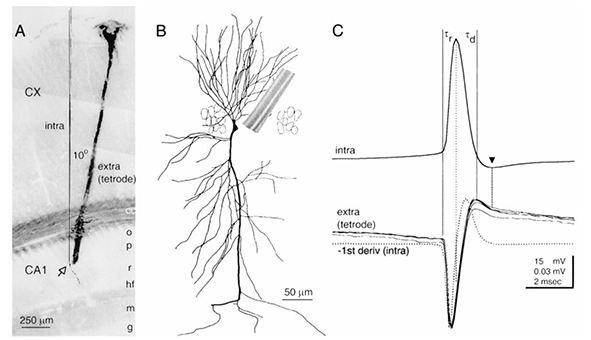
\includegraphics{Figures/Spikes/Spikes-Henze-w100-r150}
\end{center}
\caption[Intracellular and extracellular action potentials]{\textbf{Simultaneous recording of intracellular and extracellular action potentials (`spikes').}
Adapted from \citeasnoun**{Henze2000}.
\gen{Figure + caption to be updated}
}
\label{fig:Spikes:Henze}
\end{figure}
%%%%%%%%%%%

While the amplitude of the membrane-potential deflection during an action potential is about 100~mV, the amplitudes of spikes are typically less than 1~mV. Also, the shape of the spike is very different from the shape of intracellularly recorded action potentials (\Fref{fig:Spikes:Henze}). The initial sharp negative peak is often referred to as the `sodium peak' as it mainly stems from sodium ions flowing into the soma (and axon hillock) during the initial phase of the action potential. The \ghtxt{\sout{latter},later} blunter positive peak is likewise sometimes referred to as the `potassium peak'\ghtxt{,} as it is dominated by potassium ions flowing out of the soma. \gen{Dette maa vel vaere riktig aa si?} \ghnote{Hoeres riktig ut, ja.} \ghnote{Jeg har tidligere brukt kursivering for aa introduse begreper, mens du bruker fnutter. Maa bli enige om en fast konvensjon.}

When detecting spikes, the main issue is that the spike amplitude is larger than the ambient noise level, typically some tens of $\mu$V. 
%\gen{Har vi et godt tall med medhoerende referanse her?} 
%\ehnote{Tja. Ambient noise er jo veldig avhengig av forskjellige faktorer, elektrode-type og impedans, in vivo vs. in vitro, vaaken vs. bedoevet tilstand osv, valg av filter, osv.}
%\tvnnote{Alessio sa de typisk ikke tar med spikes med amplitude under 30 uV, og det var dette vi brukte i Buccino et al., 2018, J Neurophysiol, men han hadde ikke noe god kilde ellers}
For the detection of spikes, the detailed spike shape is of less importance. However, an extracellular electrode will in general measure spikes from several neurons positioned in the vicinity of the electrode contact. To obtain spike trains from individual neurons, the recorded spikes must thus be sorted in a process referred to as spike sorting~\cite**{Quiroga2007}. And in this process, the differences in spike shapes are crucial~\cite**{Einevoll2012}. Spikes shapes are also used to distinguish spikes from different neuron types. The temporal width of the spike is, for example, used to separate putative inhibitory neurons (narrow spikes) from excitatory neurons (broad spikes). But a more detailed separation into subgroups is also possible~\cite**{Buccino2018}. \ghnote{Skal vi tillate oss aa begynne setninger med And og But? Jeg synes ikke det. Foreslaar komma og liten bokstav for begge disse tilfeller.}

Detailed modeling of spikes are important for several reasons: for example, 
(i) to understand \ghtxt{\sout{what the single-neuron properties can tell us about spike shapes (and the other way around)} the relationship between single-neuron properties and spike shapes} \cite**{Holt1999,Gold2006,Pettersen2008a,Anastassiou2013},
(ii) to estimate biases regarding which types of neurons preferentially generate the spikes recorded by electrodes \cite**{Pettersen2008a},
(iii) to provide benchmarking data for development and testing of methods for spike sorting or spike-based neuron identification \cite**{Einevoll2012,CamunasMesa2013,Hagen2015,MondragonGonzalez2017,Buccino2020}, and (iv) to fit model parameters in multicompartment neuron models \cite**{Gold2007}.

%%%
\section{\blue{Recording of spikes}}
\label{sec:Spikes:recording}
Spike recordings are typically done in living brains\ghtxt{\sout{. Here}, and} the signal is obtained by high-pass filtering the extracellular potentials, with a lower cut-off set at some hundred hertz.
In contrast, the low-frequency part, the local field potential (LFP), is thought to mostly reflect synaptic inputs onto populations neurons around the contact~\cite**{Einevoll2013},
see \Fref{chap:LFP}.

A common misunderstanding is that a spike is built up only of high-frequency components. The reasoning is that\ghtxt{, since} a spike typically lasts only a couple of milliseconds and an oscillation with a period of, say, 2 milliseconds corresponds to a frequency of 500 hertz, lower frequencies will be absent or at least very weak. \ghtxt{\sout{But}However,} this is not generally true~\cite**{Pettersen2008,Schomburg2012,Ray2011,Scheffer-Teixeira2013}. Even a fast sodium spike contains frequency components with frequencies as low as 100 Hz \cite**{Pettersen2008a}. This is illustrated in Figure~\Fref{fig:Spikes:freq_dep} showing that also very narrow spikes may contain low-frequency components. In fact, a so-called $\delta$-function pulse which essentially is infinitely sharp and has zero width, is built up of equal amounts of frequency components for all frequencies.
\ghtxt{\sout{And}In addition, the sodium spike in a single neuron may coincide with} slower phenomena such as calcium spikes~\cite**{Stuart2007}, spike afterhyperpolarization \cite**{Buzsaki1988}, and \ghtxt{\sout{strongly correlated action-potential firing} spikes elicited by other neurons} \cite**{Schomburg2012}, which may further contribute to increased low-frequency components~\cite**{Buzsaki2012}. \ghnote{Uklar sistesetning. Du snakket om en spike, men listet saa opp en masse andre greier. Hvordan relaterer spiken til disse sakene i sistesetningen? Jeg gjorde et forsoek paa aa antyde det.}

%%%%%%%%%
% Figure
%%%%%%%%%
\begin{figure}[!ht]
\begin{center}
%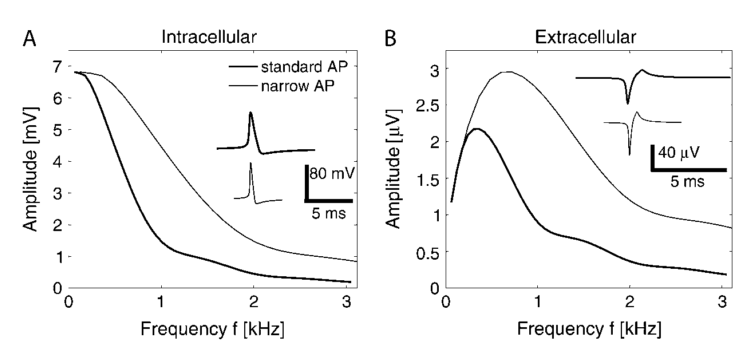
\includegraphics[width=0.6\textwidth]{Figures/Spikes/Spikes-eap_illustration.png}
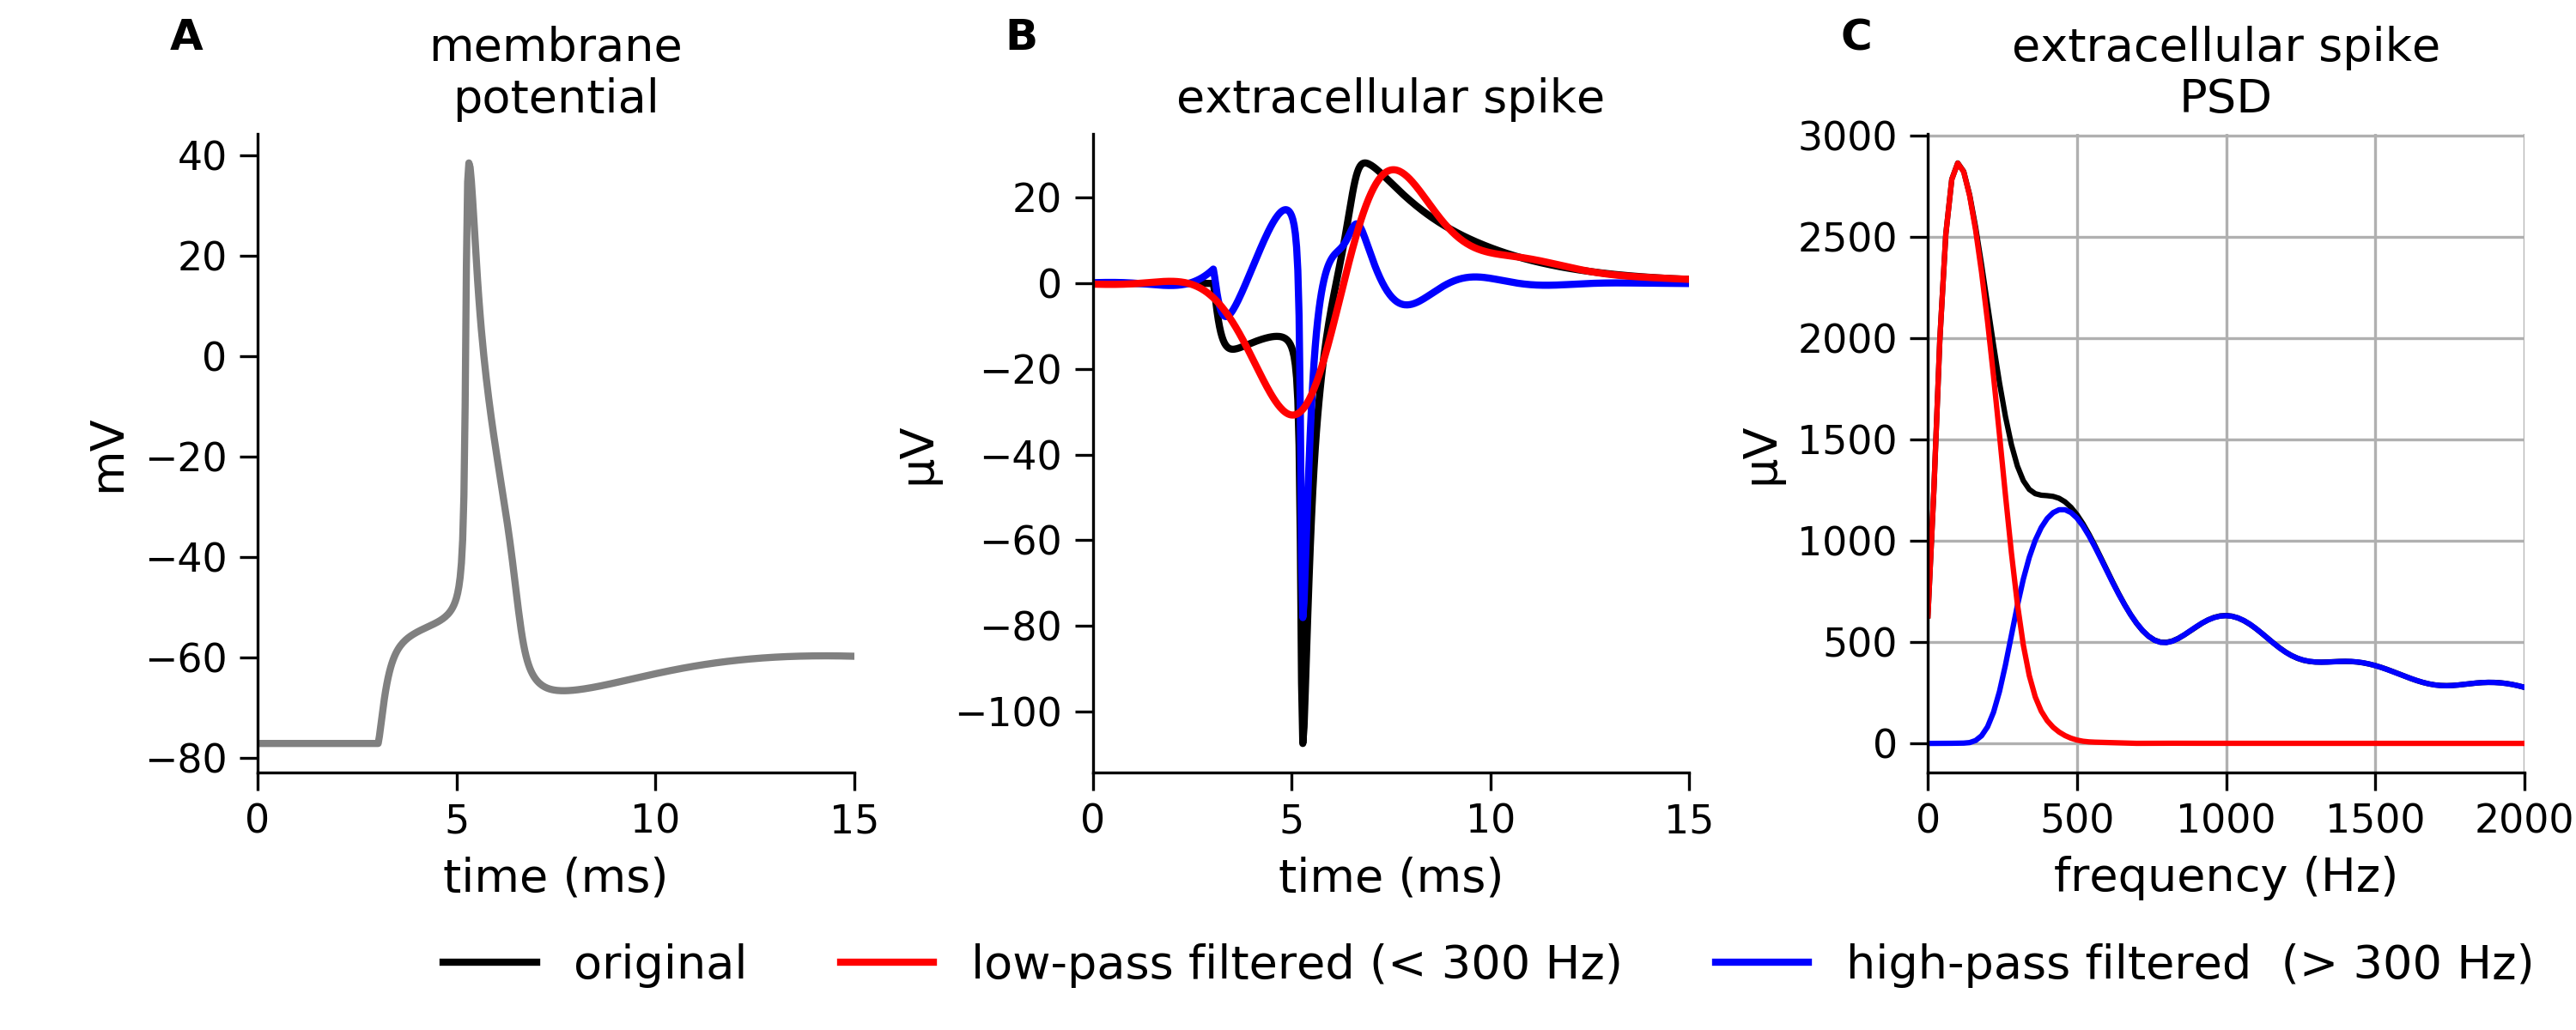
\includegraphics[width=1.0\textwidth]{Figures/Spikes/Spikes-fig_spike_freq_content_amp.png}
\end{center}
\caption[]{\textbf{Spike and frequency components.}
A: Membrane potential during firing of action potential of Hay neuron \cite**{Hay2011}. \ghnote{For aa sitere i figurtest, legg inn en klamme rett etter caption[].}
B: Corresponding extracellular spike measured \gex{XX $\mu$m} outside of soma neurons. Raw signal (black),
low-pass filtered signal (red), high-pass filtered signal (blue).
C: Frequency content of signals in B, that is, amplitudes for frequency components found by Fourier transformation.
\gen{Kanskje vi kunne legge til Fourier spektrum for intracellular action potentials ogsaa slik at vi kan kommentere
at ikke bare spike-formen i tid, men ogsaa i frekvens, er veldig forskjellig?}
\gen{Enhet paa y-akse i C maa fikses. Tar vel ogsaa bort bakgrunns-rutegrid i C?}  
}
\label{fig:Spikes:freq_dep}
\end{figure}
%%%%%

%%%%%%%%%
% Figure
%%%%%%%%%
\begin{figure}[!ht]
\begin{center}
%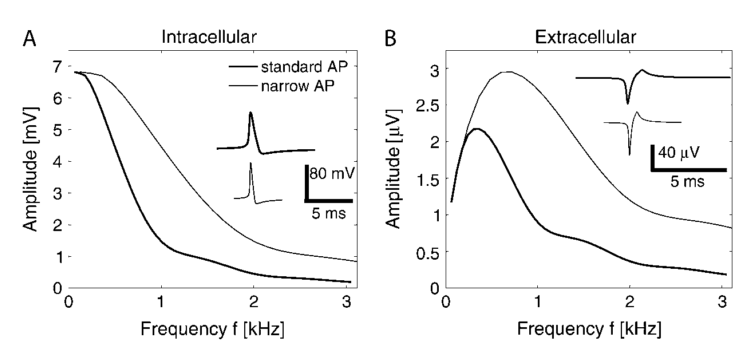
\includegraphics[width=0.6\textwidth]{Figures/Spikes/Spikes-eap_illustration.png}
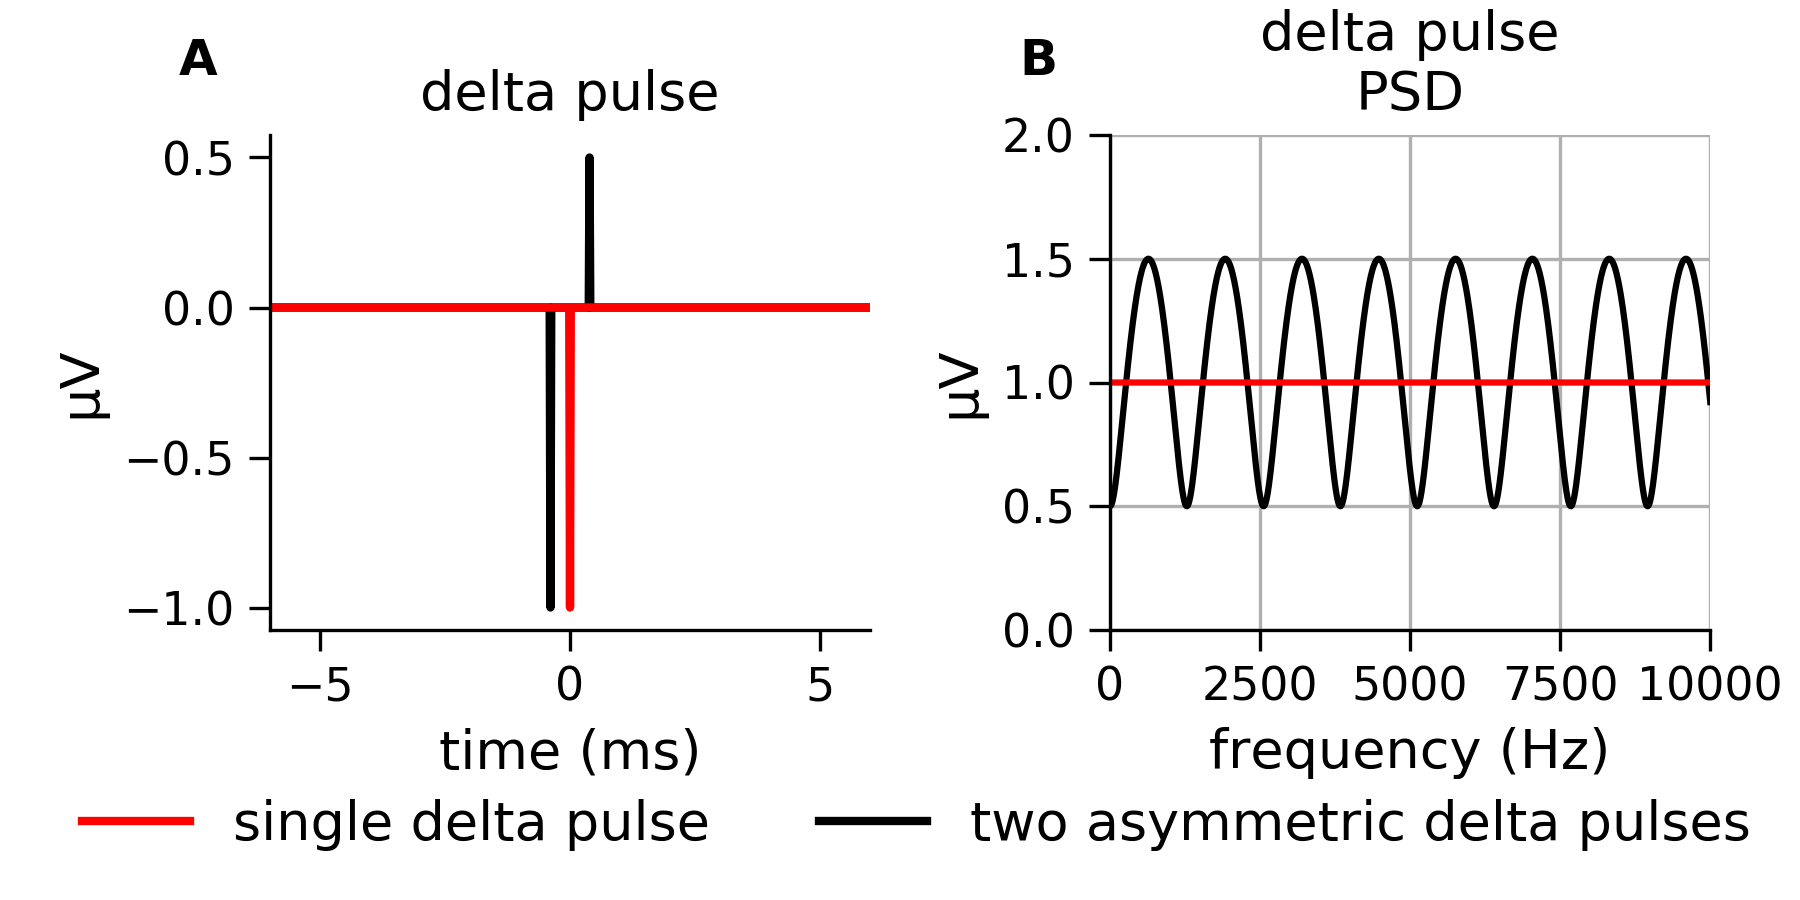
\includegraphics[width=1.0\textwidth]{Figures/Spikes/Spikes-fig_delta_pulse_freq_content.png}
\end{center}
\caption{\textbf{Delta pulses and frequency content.}
A single delta-pulse (panel A, red) has frequency components with equal contributions for all frequencies (panel B, red).
An asymmetric pair of delta-pulses, caricaturing the spike in \Fref{fig:Spikes:freq_dep}B with a negative sodium peak followed by a weaker positive potassium peak (panel A, black), instead has an oscillating frequency spectrum (panel B, black). This spectrum has its (first) maximum at 625 Hz, but also has substantial contributions from frequencies all the way down to zero.
\gen{Kanskje la x-aksen faa fra 0 till 2000 Hz som i Fig. 8.2B? Tar vel ogsaa bort bakgrunns-rutegrid i B? Enhet paa y-akse i B maa fikses. Kanskje vi kan velge -100 $mu$V som amplitude paa sodium-pulse i A slik at det ligner mer paa  Fig. 8.2?}
}
\label{fig:Spikes:freq_dep_delta}
\end{figure}
%%%

The high-pass filtering of the extracellular signal typically used in extraction of spikes from extracellular recordings, 
changes the shape and reduces the signal power of the extracellular spike signal.  The rationale for this high-pass filtering is 
not to modify the spike shape and make it more amenable for detection or spike sorting. It is rather to remove the low-frequency (LFP) part which stems from the other slower neural processes.  This LFP signal typically dominates in terms of overall power, but has very little power above a few hundred hertz~\cite**{Pettersen2008,Einevoll2013}. \ghnote{Er ikke dette en tautologi? The low-frequency part has little power in the high frequencies?}

Overviews over the challenges when measuring spikes can be found in  \citeasnoun**{Anastassiou2013} and \citeasnoun**{Whittingstall2013}.
\gen{Noen andre mulige referanser her?} 

 %%%%%%%%%%
% Figure: Spike from multi-compartment model
%%%%%%%%%%
%\begin{cnfigure}{Figures/mm/EP-spike-MultiCompartment-w100-r150}
\begin{figure}[!ht]
\begin{center}
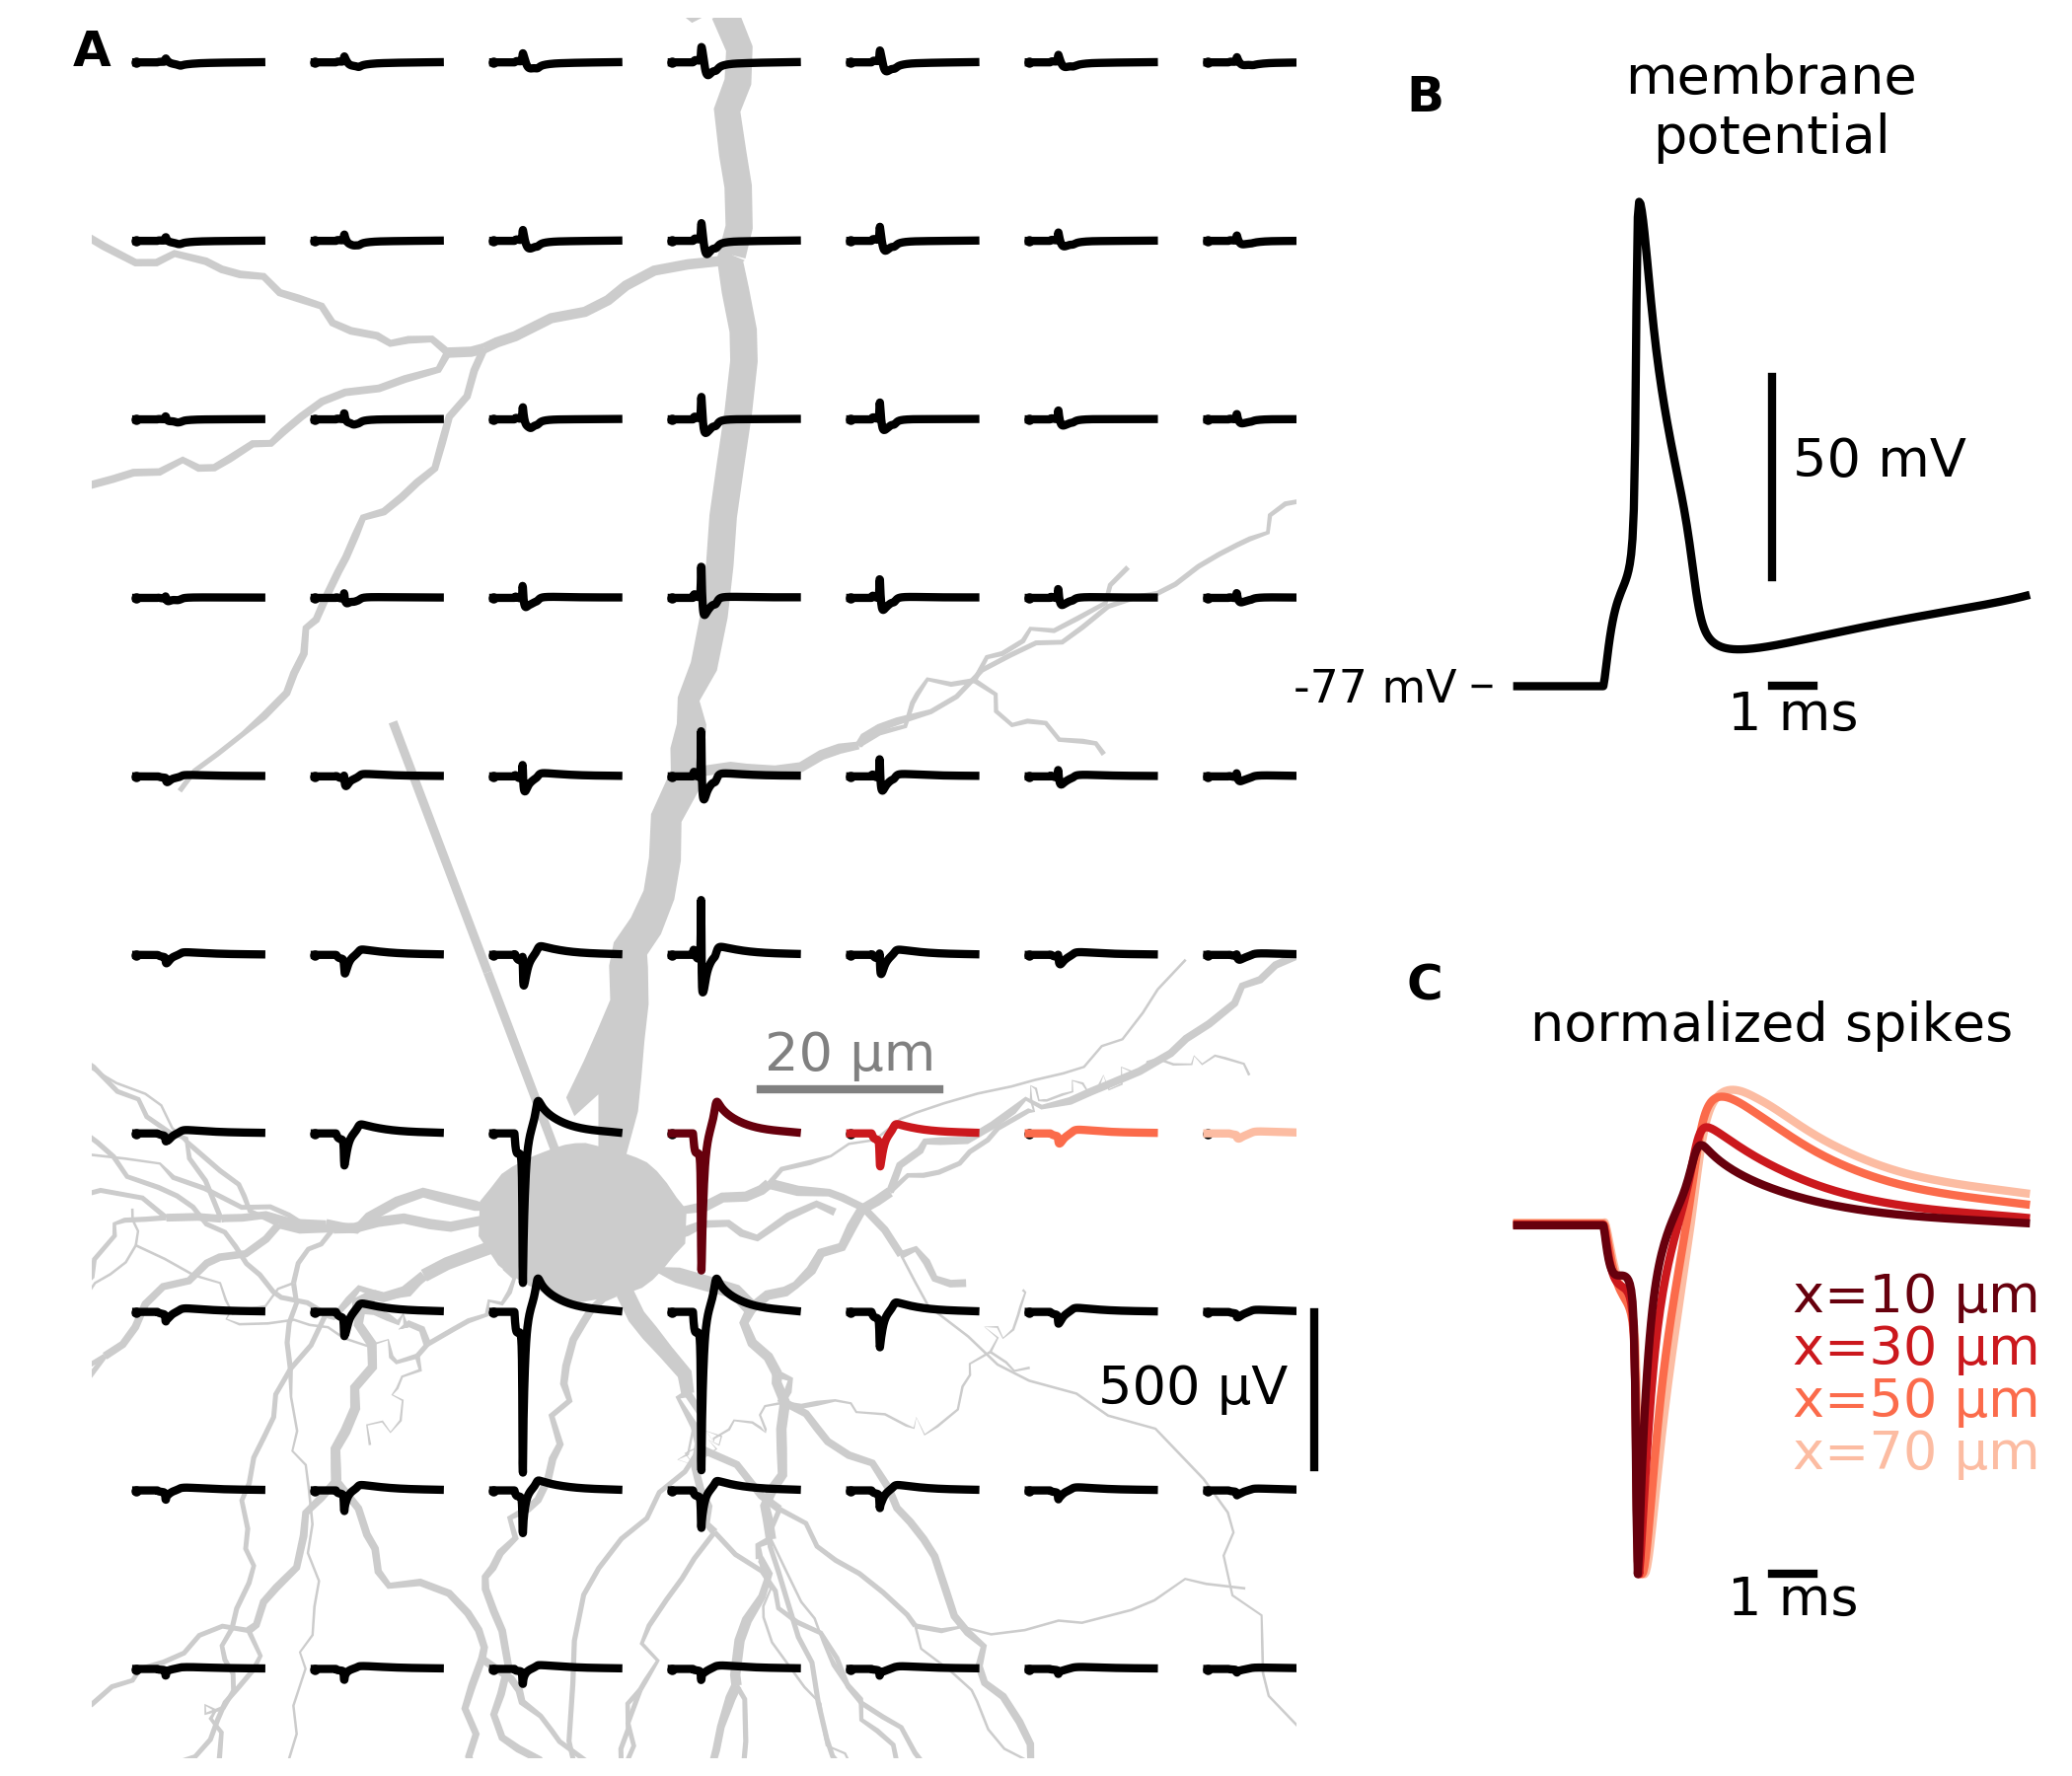
\includegraphics[width=1.0\textwidth]{Figures/Spikes/Spikes-fig_hay_eap_simpler}
\end{center}
\caption[]{\textbf{Spike from action potential for a multi-compartmental neuron model.}
A: Spikes computed at different positions around example Hay-neuron \cite**{Hay2011} using \gex{Eq. XX}.
B: Corresponding membrane potential. C: Spike shapes at different lateral positions in A as depicted by colouring. Spike shapes
are normalized to have the same magnitude of the negative peak.
The action potential was generated by injection of synaptic currents into the soma of the model neuron. 
\ehnote{Figure adapted from Fig4. i Hagen2015 kanskje? Aksonet peker i "feil" retning ogsaa. 
Det boer nevnes hva som driver depolariseringen, ser ut som en step current?}
\tvnnote{Vi ville ha en litt enklere versjon enn Fig. 4 i Hagen2015, men enig i at vi kanskje boer vurdere aa fikse retningen til axonet. Har du koden for dette? Stimuli er foreloebig synaptisk input i soma} \ghnote{Denne figuren er panel A i neste figur. Foreslaar at den fjernes, og at vi refererer dit.}
}. 
%Active sodium
%and potassium conductances in the soma compartment and computed from 
%\Fref{XX:equation:Ve-multi-compartment}.
%Left panel shows the EP at different spatial positions, while right panel shows the corresponding
%soma membrane potential during the action potential. 
%\gen{Figure + caption to be updated. Change to Hay-model,}
\label{fig:Spikes:MultiCompartment}
%\figpermOurs
\end{figure}

%%%
\section{\blue{Spikes from multi-compartment neuron models}}
\label{sec:Spikes:multi-compartment}
%%%
\ghnote{Forslag: Sec 8.2, 8.3, 8.4.1 slaas sammen til delkapitler i 8.2. som heter modeling spikes eller noe. Formaal er aa vise eksempelsimuleringer for ulike morfologier. Analysen kommer senere i nytt 8.3. og er der for enkelhets skyld i stor grad basert paa ball-and-stick. 8.3. kan gjoeres litt mer up-front med tanke paa introdusering av Fourier-greier, og vi kan referere dit i 8.1 der vi viser Fourier-resultater uten aa ha introdusert teorien. Evt. kan vi introudsere Fourier tidligere et sted, feks. i VC-kapittelet eller som eget kapittel?}
Unlike the intracellular somatic action potential which has a quite standardized appearance, the spike shapes and amplitudes can vary strongly depending on the position at which \ghtxt{\sout{it is}they are} recorded.  This is illustrated in \Fref{fig:Spikes:MultiCompartment} showing computed spikes at various positions around a neuron during the firing of an action potential. Here the scheme described in Chapter \gex{XX} is used with a biophysically detailed neuron model for a layer-5 pyramidal cell. One striking feature is the rapid decay of spike amplitude with distance from the soma. Another is the changing shape of the spike highlighted in panel C: The sharpest spikes are seen for recording close to the soma. This blunting, or low-pass filtering, of the spike with distance stems from the cable properties of the neuron, and has been referred to as `intrinsic dendritic filtering' \cite**{Linden2010,Pettersen2012} (as opposed to, say, possible filtering by the extracellular medium itself~\cite**{Bedard2012}). The origin of this intrinsic dendritic filtering effect is described below in \Fref{sec:Spikes:ball-and-stick}.

%A more detailed picture of spike shapes is obtained by considering a detailed multi-compartmental neuron model
%with a comprehensive branching structure typical for real neurons as in Figure~\Fref{fig:Spikes:MultiCompartment}.
%With this dendritic morphology the membrane currents through the dendrites are spread over a larger membrane area.
%As a result, \Fref{XX:equation:Ve-multi-compartment} predicts that the largest EP spikes will be seen
%around the soma for the example pyramidal neuron in Figure~\Fref{fig:Spikes:MultiCompartment}.  
%Around the apical dendrites, the spikes will still have an inverted shape compared to spikes close to the soma. 
%However, their amplitudes will be small, only a few microvolts, so they will not be seen in most experiments.
%
%As for the two-compartment spike model, the spike amplitude in Figure~\Fref{fig:Spikes:MultiCompartment} 
%decays sharply with distance from the neuron. In addition, the spike width increases
%with distance as demonstrated by the insets at two example positions. For the large spike recorded next to
%the soma the half-width of the spike is $\sim$0.6~ms, while at the position outside the dendrite, the half-width is increased to
%$\sim$0.7~ms. This corresponds to a low-pass filtering in the sense that the distant EP has lost some 
%high-frequency components compared to the EP close to the soma. This filtering effect is absent for the spike generated by the 
%two-compartment neuron model, and reflects that the cable properties of dendrites are important in determining 
%also the shape of recorded spikes.   
%
%*******



%%%
\section{\blue{Spikes from two-compartment neuron model}}
\label{sec:Spikes:two-compartment}
%%%
To what extent can the qualitative features regarding the position dependence of spikes seen 
in \Fref{fig:Spikes:MultiCompartment} be explained by simpler neuron models? 
While intracellularly recorded action potentials can be modelled with a single-compartment neuron model, 
the two-compartment model model is the simplest neuron model that can provide an extracellular spike at all. 
An example of a spike generated by such a model is shown in Figure~\Fref{fig:Spikes:DifferentNeuronModels}D. Around the soma, characteristic spikes with a sharp negative peak followed by a slower positive hump are seen, in accordance with typical experimental spike recordings as exemplified in Figure~\Fref{fig:Spikes:Henze}. The same spikes with inverted form are observed outside the dendrite compartment. Such inverted spikes are rarely, if ever, seen in experiments, however. This suggests that while the two-compartment model can account for large spikes recorded next to the soma, it is inadequate for 
predictions of  the detailed spatial pattern of spike shapes that would be recorded by an electrode at different positions around a neuron.   

Spike amplitudes in the two-compartment model are seen to decay with distance as in the multi-compartment model. However, the two-compartment predictions differ in that the spike shape (panel D, bottom) does not depend on position ( \ghtxt{\sout{except for possibly a complete inversion}except for the complete inversion when crossing the lateral symmetry plane of the neuron}). This can be readily understood from the two-compartment cable equation circuit \gen{Synes vi boer gaa gjennom denne modellen et sted i teorien slik at vi kan
refere til den her ...}. \ghnote{Vi har vaert inne paa det i NEURON, men vil du ha et helt delkapittel i NEURON om tokompartmentmodell med komplette ligninger?} The transmembrane current (including the capacitive current) that enters the soma compartment must at all times equal the transmembrane current leaving the dendrite compartment. The spike will thus be set up by the sum of two monopolar contributions with the same magnitude and opposite signs, and the only feature that will vary with spike position is the net amplitude of the spike. The shape of the spike will always be the same. \ghnote{Provided that there is no extracellular filtering? Evt: When the extracellular condictivity is constant, as assumed here, the shape of the spike will....}

%%%%%%%%%%
% Figure: Spikes from two-compartment, ball-and-stick and multicompartment
%%%%%%%%%%
%\begin{cnfigure}{Figures/mm/EP-spike-TwoCompartment-w100-r150}
\begin{figure}[!ht]
\begin{center}
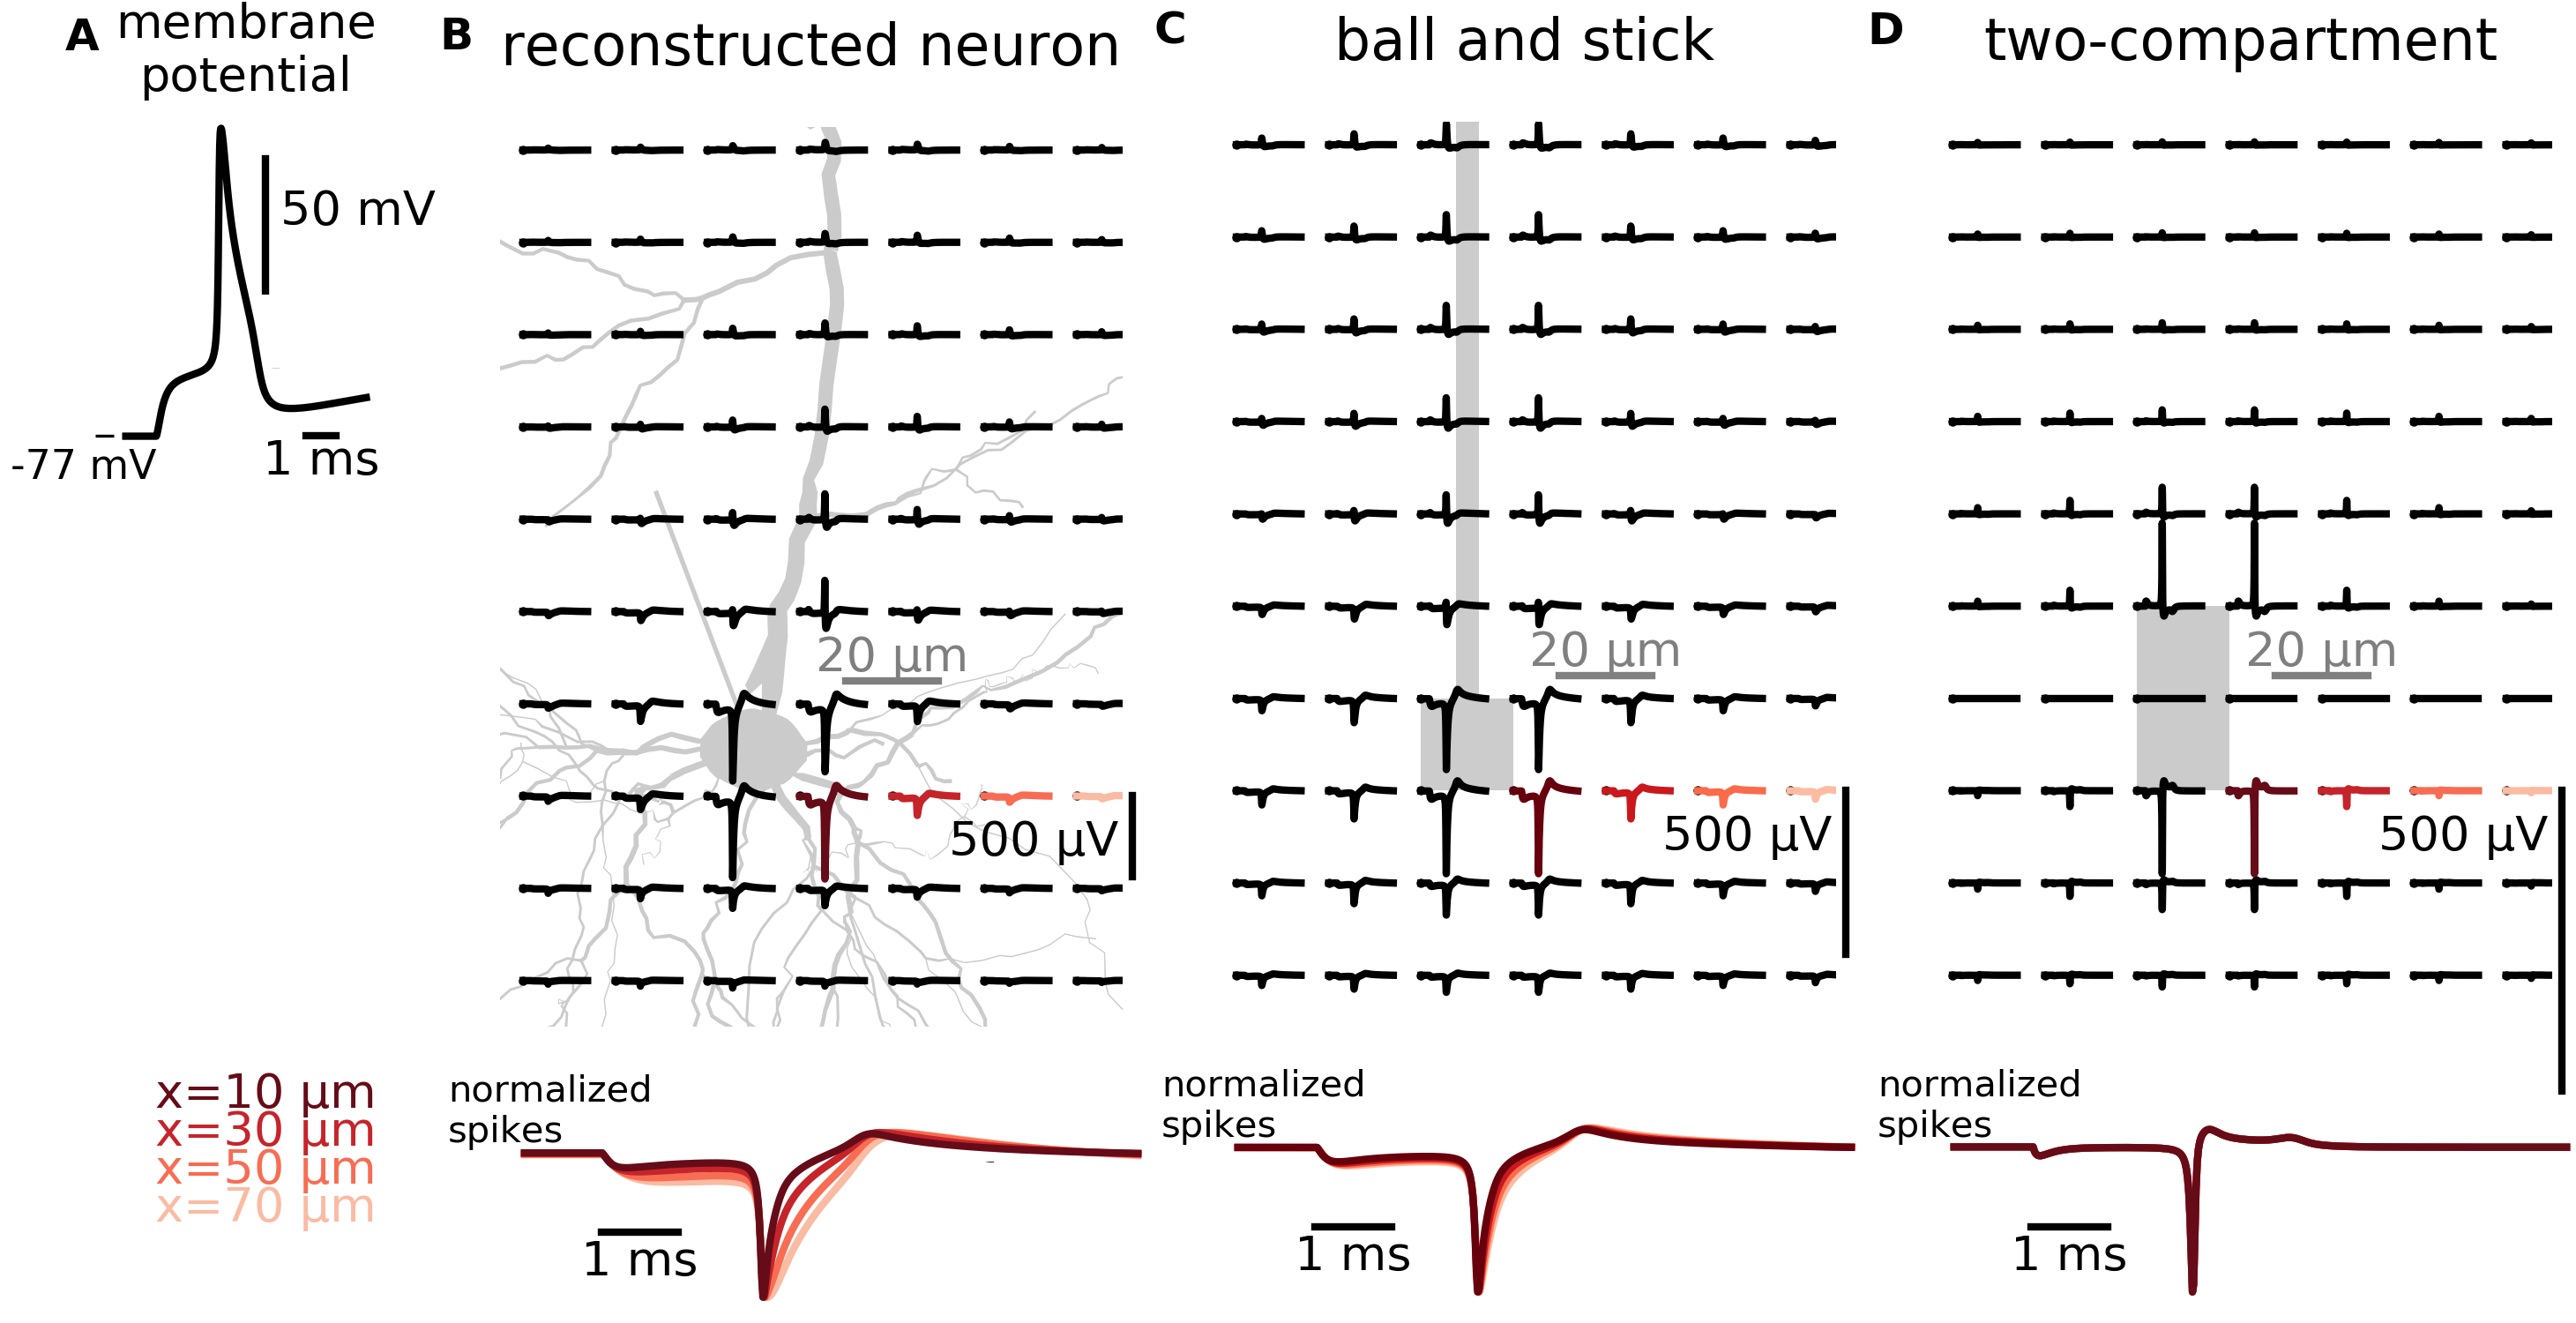
\includegraphics[width=1.2\textwidth]{Figures/Spikes/Spikes-compare_hay_bns_2c_reformat_2}
\end{center}
\caption[]{\textbf{Comparison of spikes from action potential for different neuron models.}
A: Membrane potential during spiking event, generated by injection of synaptic current into the soma of  example Hay-neuron \cite**{Hay2011}. B: Spikes computed at different positions around example Hay-neuron using \gex{Eq. XX} (top). 
C: Spikes computed for example ball-and-stick neuron when imposing the membrane potential in A in the soma of the model neuron (top). Neuron parameters are \gex{XX}. 
D: Spikes computed for example two-compartment neuron when imposing the membrane potential in A in the soma of the model neuron (top). Neuron parameters are \gex{XX}. For panels B--D, spikes shapes at different lateral positions as depicted by colouring, are shown in bottom panels. Spike shapes are normalized to have the same magnitude of the negative peak.
\gen{Lurer paa om panelene kunne blitt finere ved aa bruke et kortere utsnitt langs tidsaksen?}
}
\label{fig:Spikes:DifferentNeuronModels}
\end{figure}

%%%
\section{\blue{Spikes from ball-and-stick neuron}}
\label{sec:Spikes:ball-and-stick}
Unlike the two-compartment neuron model, the so-called ball-and-stick neuron model exhibits position dependence of the spike shape (\Fref{fig:Spikes:DifferentNeuronModels}C). In this model a dendrite cable `stick' is connected to a point-like soma.
The effect is not as pronounced as for the anatomically detailed multi-compartment neuron model (panel B),
but the key qualitative feature remains: the spike gets blunter when moving away from the soma.
In particular, the width of the negative sodium peak is seen to increase with increased lateral distance.

Unlike multi-compartment neuron models, the ball-and-stick neuron is amenable to analytical mathematical studies. 
\citeasnoun**{Pettersen2008a} took advantage of this and used this model to explore the link between the morphology and electrical properties of neurons and the shape and size of the spike they produce during an action potential. 
Figure~\Fref{fig:Spikes:ball-and-stick-results} shows the distance dependence of the spike amplitude and spike width both for a detailed multi-compartmental pyramidal neuron model and ball-and-stick neurons. While the spike width and amplitude of the multi-compartmental neuron are larger than for the two example \ghnote{Gaute da, mangler det ikke en bindestrek her?} ball-and-stick neurons (with short and long dendrite sticks, respectively), the shapes of the curves are similar. \ghnote{Kan vi ikke velge parametere slik at amplituden og shapen ligner i de to tilfellene?}  \gen{Jo, det kan sikkert vaere mulig. Dette er klippet rett fra Pettersen2008a.} Note also that the results for a ball-and-stick neuron with an infinitely long dendritic stick is
effectively identical to the long-stick results in the figure~\cite**{Pettersen2008}.


%%%%%%%%%%
% Figure: Spike widths and amplitudes
%%%%%%%%%%
%\begin{cnfigure}{Figures/mm/EP-spike-ball-and-stick-results-w100-r150}
\begin{figure}[!ht]
\begin{center}
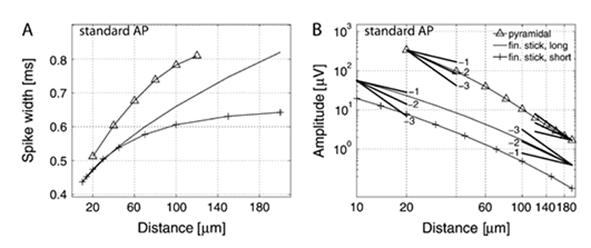
\includegraphics{Figures/Spikes/Spikes-ball-and-stick-results-w100-r150}
\end{center}
\caption[]{
Spike widths (left) and (peak-to-peak) spike amplitudes (right) as a function of distance from soma for a detailed pyramidal cell model (pyramidal) and two types of ball-and-stick models: long, finite ball-and-stick model (fin.~stick, long) with diameter $d=2~\mu$m and length $l=1$~mm and a short, finite ball-and-stick model (fin.~stick, short) with diameter $d=1~\mu$m and length $l=0.2$~mm. The intracellular action potential shown in the inset in the left panel of \Fref{fig:Spikes:ball-and-stick-frequency} was imposed as a voltage-clamp in the soma, and the size and electrical properties of the soma thus did not affect the results. The EP was recorded in the somatic plane normal to the stick/primary apical dendrite. In right panels guidelines illustrating the power-law decays $1/r$ and $1/r^{2}$ have been added. For further details see \citeasnoun**[Figure 6]{Pettersen2008}. \gen{Figure + caption to be updated.}  Adapted from \citeasnoun**{Pettersen2008}. \gen{Her kunne man jo kjoert ut nye resultater for Hay-modellen, men det er vel like greit aa bare bruke figurene fra Pettersen2008?} \tvnnote{Gaar jo forsaavidt fort aa lage paa nytt, og kan jo vaere fint at det blir en del av koden leserne har tilgjengelig?}
\gen{Enig. I tilfelle maa ogsaa Fig. 8.7 lages paa nytt.} 
}
\label{fig:Spikes:ball-and-stick-results}
%\figpermOurs
\end{figure}
%%%%


%
%%%%%%%%%%%
%% Figure: Neuron models considered in plot of spike widths and amplitudes
%%%%%%%%%%% 
%%\begin{cnfigure}{Figures/mm/EP-spike-ball-and-stick-neuron-models-w43-r300}
%\begin{figure}[!ht]
%\begin{center}
%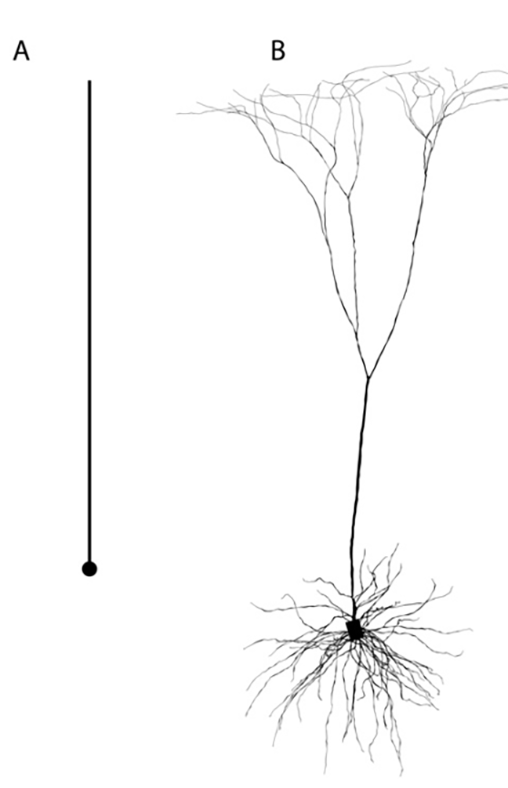
\includegraphics{Figures/Spikes/Spikes-ball-and-stick-neuron-models-w43-r300}
%\end{center}
%\caption[]{\textbf{Neuron models considered in results in Figure~\Fref{fig:Spikes:ball-and-stick-results}}. 
%\gen{Mulig vi ikke trenger en slik figur lenger pga Fig 8.3}
%Adapted from \citeasnoun**{Pettersen2008}.
%}
%\label{fig:Spikes:ball-and-stick-neuron-models}
%%\figpermOurs
%\end{figure}

\subsection{\blue{Frequency components of spikes}}
\label{sec:Spikes:Fourier}
To understand the physical origin of these results it is easier to consider each frequency component of the action potential separately. \ghnote{(1) Er "the physical origin" rett begrep? (2) Uklart hva "these results" refererer til. Ny aapningssetning trengs. To understand the physics behind the dependence of spike shape on position ... ? To analyze extracellular potentials, it is easier to ...?}  From Fourier theory it follows that any signal such as the time course of a spike $V_\mathrm{e}(t)$, can be written as a sum of waves with different frequencies. Such a Fourier sum can be constructed in various ways. The derivations presented below, building on \citeasnoun**{Pettersen2008a}, use the convention that a time signal $S(t)$ can be written as
%%%
\begin{equation}
S(t) = Re \{ \sum_{f}  \hat{S}(f) \exp (j 2 \pi f t) \}
\label{eq:Spikes:Fourier_sum}
\end{equation}
%%%
where $Re\{z\}$ represents the real part of the complex number $z$.  Here $j$ is the unit of imaginary numbers, $f$ is the frequency, and the weight $\hat{S}(f)$ is in general  complex. 

\ghnote{Jeg tror dette asnittet trenger en mer utfoerlig aapning. (1) Er det rart aa infoere dette med frequency components som underkapittel i Ball-and-stick? Ville det kanskje vaert bedre aa hatt tre oppsummerende og korte delkapitler i 8.2: 8.2.1 "Spikes from multicomp", 8.2.2. "Spikes from two-comp", 8.2.3. "Spikes from ball and stick". Og saa 8.3. Analysis of frequency components of spikes, eller noe slik, der man begynner med å introdusere Fourier, og foelger opp med en analyse som for enkelthets skyld primaert er basert paa ball-and-stick? Synes det virker som en mer logisk struktur.}

Figure~\Fref{fig:Spikes:ball-and-stick-frequency} illustrates the Fourier decomposition of the
intracellular action potential (membrane potential) and extracellular spike, respectively.
In panel B the weight of the different frequency components needed to represent the signals are shown.
A key observation here is that unlike for the intracellular action potential, the largest
contributions to the extracellular spike, comes from frequencies larger than 100~hertz.
\ghnote{Det overrasket at f-spektrum til intra vs ekstra er saa fundamentalt ulike. Er signalet i Figurpanel A ufiltrert, mens det i B er filtrert?}
\gen{Nei, dette skyldes fysikken. Extra reflekterer transmembrane stroemmer som inneholder mer av de hoeye frekvensene enn det "lav-frekvente" membran-potensialet.}
\tvnnote{De er foroevrig betydelig likere i mine simuleringer med Hay modellen, selv om det generelle moensteret vel kanskje er omtrent det samme som her.}


%%%%%%%%%%
% Figure: Action potential and its frequency content
%%%%%%%%%%
%\begin{cnfigure}{Figures/mm/EP-spike-ball-and-stick-frequency-w90-r150}
\begin{figure}[!ht]
\begin{center}
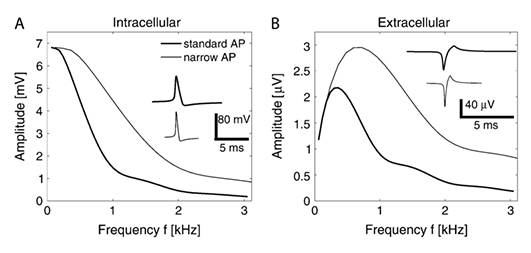
\includegraphics{Figures/Spikes/Spikes-ball-and-stick-frequency-w90-r150}
\end{center}
\caption[]{(a) Action potential used in simulations in Figure~\Fref{fig:Spikes:ball-and-stick-results}(inset) 
and its frequency content.
%The intracellular spike width is defined as the
%width of the AP at half amplitude and is 0.55~ms for the standard
%AP, and half the value for the narrow AP. 
(b) Frequency content of example extracellular spike.
Inset: Typical spike shape computed a distance $r=10~\mu$m
perpendicular to the dendrite at the level of soma for a ball-and-stick 
neuron with diameter $d=2~\mu$m and infinite dendrite length.
Here the intracellular action potential in left panel was imposed as a voltage-clamp in the soma.
The extracellular spike width is defined as the width of the negative phase at 25\% of its maximum
amplitude and is 0.44~ms for the example spike.
The amplitude (peak-to-peak value) of the spike is $56~\mu$V  
\gen{Figure + caption to be updated. Will only include standard AP in final figure.} 
Adapted from \citeasnoun**{Pettersen2008}.}
\gen{Her kunne man jo kjoert ut nye resultater for Hay-modellen, men det er kanskje like greit aa bare bruke figurene fra 
Pettersen2008?} \ghnote{mV/Hz paa y-aksen.}
\label{fig:Spikes:ball-and-stick-frequency}
%\figpermOurs
\end{figure}

%\subsection{Frequency-dependent electrotonic length constant}
%\label{sec:Spikes:Fourier}
%
%For the ball-and-stick neuron, a membrane current entering the soma has to return to ECS through the cable stick, see Figure~\Fref{fig:Spikes:ball-and-stick-sketch}. When an oscillating membrane current is entered through the soma, the spatial pattern of return current will depend on the frequency of the oscillation due to the capacitive properties of the membrane: For higher frequencies the capacitive membrane current will be larger, and the 
%membrane effectively more leaky. Thus the injected soma current will return closer to the soma for higher frequencies, 
%as  seen in the inset in Figure~\Fref{fig:Spikes:ball-and-stick-sketch}.  

\subsection{\blue{Approximate spike formulas}}
\label{sec:Spikes:approximate}
To compute the extracellular spike generated by an imposed oscillatory current, \ghnote{Tung start. Hva er en imposed oscillatory current? Det er et AP dekomonert i ulike frekvenser og matet inn som en soma-stroem, regner jeg med. Boer forklare dette tydeligere.} the stick must be divided into small compartments  and the multi-compartmental formula in Equation \gex{XX} used. This in general requires detailed knowledge of the resulting membrane currents in all compartments. 
While these can be computed for the ball-and-stick neuron (see, for example, \citeasnoun**{Pettersen2014}), 
the resulting formula for the spike becomes cumbersome and difficult to interpret.  However, some useful insights can be obtained in two limiting cases: the recording being very near to the soma or very far from the soma.

%For recording positions very close to the soma, the contribution from the soma current will dominate 
%in the sum in \gex(XX). In this case the distance from the electrode
%to the return currents in the dendrite will be much larger than the distance to soma. 
%
%%
%With only the contribution from
%the soma compartment included, the amplitude $|\hat{V}_\mathrm{e,near}(f,\vec{r})|$  
%of the EP signal for each Fourier component with frequency $f$ is found to be

\subsubsection{Spikes recorded near the soma}
\label{sec:Spikes:near-spikes}
\tvnnote{En del bruker den deriverte av membranpotensial til aa approksimere spikes. Boer det taes med?}
\gen{Ja, det kommenteres naa lenger ned i "Spike shape dependence on distance".}
To understand the dependence of spike shapes and amplitudes on model parameters for the ball-and-stick neuron, it is useful
to consider the extracellular potentials set up by each of the frequency (Fourier) components of the action potentials separately. \ghnote{Noe ala setningen over burde kanskje staa skrevet ut litt mer utfoerlig i begynnelsen av "Frequency components of spikes"}
For recording positions $\vec{r}$ very close to the soma, the contribution from the soma current will dominate over the contributions from the dendrite 
in the sum giving the extracellular potential in Equation \gex{XX}. Then the amplitude of the
predicted oscillating extracellular potential $|\hat{V}_\mathrm{e,near}(f,\vec{r})|$ is approximately given by 
%
\begin{equation}
  |\hat{V}_\mathrm{e,near}(f,\vec{r})| = \frac{|\hat{I}_\mathrm{s}(f)|}{4 \pi \sigma r} 
  \label{eq:Spikes:Ve_near_1}
\end{equation}
%
where $|\hat{I}_\mathrm{s}(f)|$ is the amplitude of the oscillating current through the soma membrane.
%and also the axial current entering the dendrite from the soma compartment. 
For the relatively high frequencies of most relevance for the spike, this soma current is related to the soma membrane potential 
$\hat{V}_\mathrm{s}(f)$ through~\cite**{Pettersen2008a}
%
\begin{equation}
  |\hat{I}_\mathrm{s}(f)| =  \frac{\pi^{3/2} d^{3/2}}{\sqrt{2}} \sqrt{ \frac{f C_\mathrm{m}}{R_\mathrm{a}} }  |\hat{V}_\mathrm{s}(f)|
  \label{eq:Spikes:Isoma}
\end{equation}
%
and the contribution to the spike is thus found to be
%
\begin{equation}
  |\hat{V}_\mathrm{e,near}(f,\vec{r})| 
  = \frac{\sqrt{\pi}}{4 \sqrt{2} \sigma}
     \frac{d^{3/2}}{r} 
     \sqrt{ \frac{f C_\mathrm{m}}{R_\mathrm{a}} }  |\hat{V}_\mathrm{s}(f)| 
  \propto \frac{d^{3/2}}{r} \sqrt{ \frac{f C_\mathrm{m}}{R_\mathrm{a}} }  |\hat{V}_\mathrm{s}(f)| 
  \label{eq:Spikes:Ve_near_2}
\end{equation}
%
%%%%%%%%%%
%However, as shown in XX
%Box~\Fref{mm:box:ball-and-stick-spikes} 
%some useful insights can be obtained in two limiting cases: the recording being very near to the soma or very far from the soma.

%For recording positions very close to the soma, the contribution from the soma current will dominate 
%in the sum in \Fref{XX:equation:Ve-multi-compartment}. In this case the distance from the electrode
%to the return currents in the dendrite will be much larger than the distance to soma. With only the contribution from
%the soma compartment included, the amplitude $|\hat{V}_\mathrm{e,near}(f,\vec{r})|$  
%of the EP signal for each Fourier component with frequency $f$ is found to be
%%
%\begin{equation}
%  |\hat{V}_\mathrm{e,near}(f,\vec{r})| 
%  \propto \frac{d^{3/2}}{r} \sqrt{ \frac{f C_\mathrm{m}}{R_\mathrm{a}} }  |\hat{V}_\mathrm{s}(f)| 
%  \label{eq:Spikes:Ve_near}
%\end{equation}
%%
The suffix `near' is added because this expression only applies in the `near-field' limit, that is,
close to the soma.
$|\hat{V}_\mathrm{s}(f)|$ is the amplitude of Fourier component of the soma membrane potential at the same
frequency (see Figure~\Fref{fig:Spikes:ball-and-stick-frequency}). Further, $d$ is the diameter of the dendritic
stick, $C_\mathrm{m}$ is the specific membrane capacitance, and $R_\mathrm{a}$ is the specific axial resistance.  

%One of the predictions from the formula in \Fref{eq:Spikes:Ve_near_2} is that the amplitude of each Fourier component decays
%as $1/r$ when moving away from soma (yet staying within distances where the `near-field' approximation is still applicable).
%Since this applies to all Fourier components which together constitute the action potential, this implies that the amplitude of the 
%spike will decay as $1/r$ in this regime as well.
%\gen{From David Sterratt: Intuition for the relationship witd $d, C_m, f, r_a$.}

%%%%%%%%%%
% Figure: Frequency-dependent distribution of return currents
%%%%%%%%%%
%\begin{cnfigure}{Figures/mm/EP-spike-ball-and-stick-sketch-w70-r300}
\begin{figure}[!ht]
\begin{center}
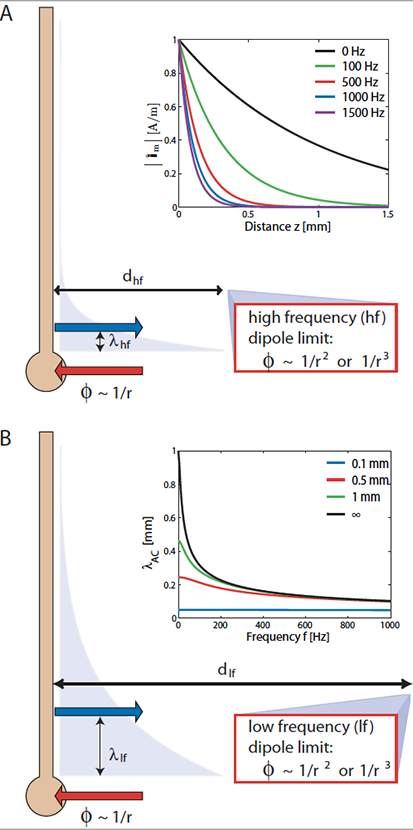
\includegraphics{Figures/Spikes/Spikes-ball-and-stick-sketch-w70-r150}
\end{center}
\caption[]{Illustration of ball-and-stick neuron and its frequency-dependent 
distribution of dendritic return currents following injection of a sinusoidal current into the soma.
The net current entering the soma will enter the dendrite as an axial current, and return to the 
ECS via the dendrite membrane. The inset shows the spatial distribution of this return current
for different frequencies. The higher the frequency, the closer the return currents will be and
the smaller the frequency-dependent length constant $\hat{\lambda}(f)$, reflecting the weighted mean 
of the return-current positions (see sidebox), will be. 
\gen{Figure + caption to be updated.} Adapted from \citeasnoun**{Pettersen2012}.
}
\label{fig:Spikes:ball-and-stick-sketch}
%\figpermOurs
\end{figure}
%


\subsubsection{Spikes recorded far away from soma}
\label{sec:Spikes:far-spikes}

For spikes recorded close to the soma, a single membrane current, the soma current,
dominates the sum in Equation \gex{XX}. 
For recording positions far away from the soma, the contribution from return membrane currents must also be included in the sum. For the ball-and-stick neuron, a membrane current entering the soma has to return to ECS through the cable stick, see Figure~\Fref{fig:Spikes:ball-and-stick-sketch}. When an oscillating membrane current enters through the soma, the spatial pattern of return current will depend on the frequency of the oscillation due to the capacitive properties of the membrane: For higher frequencies the capacitive membrane current will be larger, and the membrane effectively more leaky. Thus the injected soma current will return to the extracellular space 
closer to the soma for higher frequencies, as  seen in the inset in Figure~\Fref{fig:Spikes:ball-and-stick-sketch}.  

An approximate way of including the contribution to the spike from the dendritic return currents is to
assume all return currents to leave the dendrite at a single point on the dendrite. Then we are left with
a current dipole where the transmembrane current entering at the soma is at all times balanced by an oppositely directed current
with the same magnitude leaving at a single point on the dendrite. The current dipole length is then given by the distance
between the soma and the dendritic position of the return current. 

As shown in Figure~\Fref{fig:Spikes:ball-and-stick-sketch} this current dipole length will depend on frequency.
A natural choice is to choose the dipole length to be equal to the frequency-dependent length constant $\lambda_\mathrm{AC}(f)$ of the stick,
where the length constant corresponds to the mean value of the 
envelope of the sinusoidally varying (normalized) membrane current
$\hat{i}_\mathrm{m}$ weighted with distance $z$ from soma, see Figure~\Fref{fig:Spikes:ball-and-stick-sketch}. 
For an infinite dendrite stick this corresponds to
%
\begin{equation}
  \lambda_\mathrm{AC}^\infty(f) = \frac{\int_0^\infty z |\hat{i}_\mathrm{m}| dz}{\int_0^\infty |\hat{i}_\mathrm{m}| dz} 
  \label{eq:Spikes:formula_lambda_ac}
%=  \frac{\sqrt{2}\lambda}{\sqrt{\sqrt{W^2+1}+1}}.
\end{equation}
%
For high frequencies ($f \gg 1/2 \pi R_\mathrm{m} C_\mathrm{m}$) this is after some algebra 
found to give (see \citeasnoun[Appendix C]{Pettersen2008a} for details)
%
\begin{equation}
 \lambda_\mathrm{AC}^\infty(f) =  \frac{\lambda}{\sqrt{\pi f \tau}} = 
  \frac{1}{2\sqrt{\pi}} \sqrt{\frac{d}{f R_\mathrm{m} C_\mathrm{m}}}
\label{eq:Spikes:approx_lambda_ac}
\end{equation}
%
where $\lambda$ is the cable length constant from Equation~\gex{XX}.


Then the extracellular potential contribution from each frequency component can be approximated by using the 
dipolar expression in Equation~\gex{XX}, that is,
%%%
\begin{equation}
  |\hat{V}_\mathrm{e,far}(f,\vec{r})| =  \frac{|p(f) \cos \theta|}{4 \pi \sigma r^2} 
                                            = \frac{| \hat{I}_{s}(f) \lambda_\mathrm{AC}(f) \cos \theta|}{4 \pi \sigma r^2}   
                                                                                        \label{eq:Spikes:Ve_far_1}
\end{equation}
%Chapter~\Fref{XX:chap:XX}
Thus for spikes measured far away from the soma we find 
%  
\begin{equation}
  |\hat{V}_\mathrm{e,far}(f,\vec{r})|  = \frac{1}{8 \sqrt{2} \sigma} d^{2} \frac{1}{r^2  R_\mathrm{a}} 
      |\hat{V}_\mathrm{s}(f) \cos \theta | 
  \propto d^{2} \frac{|\cos \theta|}{r^2  R_\mathrm{a}} |\hat{V}_\mathrm{s}(f)| 
  \label{eq:Spikes:Ve_far_2}
\end{equation}
The suffix `far' is added because this expression only applies in the `far-field' limit, that is,
far away from the soma. 
%
%Equations~(\Fref{eq:Spikes:Ve_near_2}) and (\Fref{Spikes:box:equation:Ve_far_2}) describe how each frequency component of 
%the soma membrane potential  $\hat{V}_\mathrm{s}(f)$ is `translated' into frequency components of the 
%EP spike ($\hat{V}_\mathrm{e,near}(f,\vec{r})$ and $\hat{V}_\mathrm{e,far}(f,\vec{r})$, respectively). 
%%\end{boxfloat}
%%%%%%%%%%%%%%%%%%%%%%%%%%%%%%%%%%%%%%%%%


%An estimate of this length is provided by the 
%frequency-dependent length constant  $\lambda_\mathrm{AC}(f)$  corresponding to the weighted mean of the positions of the return currents along
%the dendrite stick (see Box XX). 
%Then with the use of expression for the EP around a current dipole in 
%\Fref{XX:equation:Ve-dipole-p}:
%%%%
%\begin{equation}
%  |\hat{V}_\mathrm{e,far}(f,\vec{r})|  \propto d^{2} \frac{|\cos \theta| }{r^2  R_\mathrm{a}}  |\hat{V}_\mathrm{s}(f)| 
%  \label{eq:Spikes:Ve_far}
%\end{equation}
%%%%



%A first observation from this formula is that the EP is no longer radially symmetric, and depends both on the radial distance $r$ from the neuron and  the angle $\theta$ with the dipole axis, that is, the direction of the dendritic stick.
%The amplitude will be largest above and below the neuron where $\theta=0^\circ$ and $\theta=180^\circ$, respectively. In the sideways direction 
%($\theta \sim 90^\circ$) the EP will be much smaller, as is characteristic for spatial pattern of potentials around a current
%dipole as illustrated in Figure~\Fref{fig:Spikes:TwoCompartment}. A qualitatively similar dipolar pattern, although not so distinct,
%is also seen for the spike generated by the biophysically detailed multi-compartment neuron in Figure~\Fref{fig:Spikes:DifferentNeuronModels}.


%Another difference of this far-field expression with the near-field expression in \Fref{eq:Spikes:Ve_near}, is that the
%amplitude decays as $1/r^2$, characteristic for potentials around dipolar sources, rather than $1/r$ which is characteristic for potentials around 
%a single source. This transition from a $1/r$ `monopolar' regime to a $1/r^2$ dipolar regime is indeed observed in
%the spike-amplitude panel in Figure~\Fref{fig:Spikes:ball-and-stick-results}.

\subsection{\blue{Spike amplitude dependence on distance}}
A prediction from the near-field formula in \Fref{eq:Spikes:Ve_near_2} is that the amplitude of each Fourier component decays as $1/r$ when moving away from the soma, 
as long as the position remains within distances where the `near-field' approximation still applies.
Since this applies to all frequency components which together constitute the action potential, this implies that the amplitude of the 
spike will decay as $1/r$ in this regime as well. 

Far away, the far-field formula \Fref{eq:Spikes:Ve_far_2} implies that the spike amplitude depends not only on the radial distance $r$ from the neuron, but also the angle $\theta$ with the dipole axis, the direction of the dendritic stick. The amplitude will be largest above and below the neuron where $\theta=0^\circ$ and $\theta=180^\circ$, respectively. In the sideways direction 
($\theta \sim 90^\circ$) the spike will be much smaller, as is characteristic for spatial patterns of potentials around a current
dipole as illustrated in Figure~\Fref{fig:Spikes:DifferentNeuronModels}D. A qualitatively similar dipolar pattern, although not so distinct,
is also seen for the spike generated by the biophysically detailed multi-compartment neuron in 
Figure~\Fref{fig:Spikes:DifferentNeuronModels}.
Another difference of this far-field expression with the near-field expression in \Fref{eq:Spikes:Ve_near_2}, is that the
amplitude decays as $1/r^2$, characteristic for potentials around dipolar sources, rather than $1/r$ which is characteristic for potentials around 
a single source. %This transition from a $1/r$ `monopolar' regime to a $1/r^2$ dipolar regime was also found in model studies with biophysically detailed 
%neurons \cite[Fig.~X]{Pettersen2008}.
%\todo{Connect to Figure :EP-spike-ball-and-stick-results}

An overall observation is that the spike is quite local, with the amplitude of the spike decaying rapidly with distance from the neuron soma. 
For the pyramidal neuron considered in Figure~XX, for example, the spike amplitude decays from about
300 microvolts a distance 20 micrometers from the soma centre to only about 10 microvolts a
distance 100 micrometers away. \gen{Update when new figures are added}
This rapid decay eases the interpretation of recorded spikes, since it implies
that in practice an electrode contact will only pick up spikes from neurons with somas positioned within a radius of some tens of micrometers.
%\todo{GTE: Rewrite this to compare with our own figure spikes around multicompartmental model + refer to Pettersen2008}  

%\paragraph{Spike amplitude dependence on neuronal parameters}
\subsection{\blue{Spike amplitude dependence on neuronal parameters}}
The spike amplitude is proportional to $d^{2}$ far away from the soma and to $d^{3/2}$ close to the soma,
where $d$ is the diameter of the dendritic stick diameter. This implies that far away from the soma the spike amplitude is proportional to  the cross-sectional area of the dendrite. Close to the soma, the spike amplitude also increases with dendrite diameter, but slightly less so.

Another observation is that the spike amplitude is independent of the membrane resistance $R_\mathrm{m}$ of the dendrite.
This reflects that the frequencies dominating the spike are so high that the ionic membrane current, governed by $R_\mathrm{m}$, is
much smaller than the capacitive membrane current, governed by membrane capacitance $C_\mathrm{m}$.  
Thus the spatial distribution of the return current along the dendrite will depend only on the capacitive current. This dependence
is seen through the presence of  $C_\mathrm{m}$ in the near-field formula in \Fref{eq:Spikes:Ve_far_2}. 
Note that in the far-field formula \Fref{eq:Spikes:Ve_far_2},  $C_\mathrm{m}$ is absent due to cancellation with another factor containing $C_\mathrm{m}$ in the mathematical derivation, 
cf. \citeasnoun[Equation 23]{Pettersen2008}.)

In Equations~\Fref{eq:Spikes:Ve_near_2} and \Fref{eq:Spikes:Ve_far_2}, the spike amplitude is reduced when the 
axial resistance $R_\mathrm{a}$ in the dendrites is increased. This reflects that an increased axial resistance implies that the current entering
the soma during the first phase of an action potential will return closer to the soma. This implies shorter distances on average between the sink (soma) and the sources, where the current return to the ECS, and thus a smaller current dipole and a smaller spike.


\subsection{\blue{Spike shape dependence on distance}}
The near-field and far-field formulae in \Fref{eq:Spikes:Ve_near_2} and \Fref{eq:Spikes:Ve_far_2} respectively also give qualitative insights regarding the shape of the spike. In the near-field expression, the high-frequency components of the spike is amplified 
compared to the low-frequency components, with $\hat{V}_\mathrm{e,near}(f,r) \propto \sqrt{f}$.
Thus close to the soma the spike is observed to be sharper than the intracellular action potential,
as observed in the insets in Figure~\gex{XX}. \gen{If we include such in new figures.} 
In the far-field regime there is no such high-frequency amplification ($\hat{V}_\mathrm{e,near}(f,r) \propto f^0 \sim 1$).
As a consequence, spikes measured far away from the soma will have less high-frequency content than those measured close to soma.
Thus the far-away spikes will be blunter and have larger spike widths as seen in the spike-width panel of 
Figure~\Fref{fig:Spikes:ball-and-stick-results}.

At times, the time-derivative of the membrane potential has been used as a proxy for the shape of the extracellular spike.
This would correspond to  $\hat{V}_\mathrm{e}(f) \propto f$ as a time derivation of a Fourier component   
$\exp (j 2 \pi f t)$  is proportional to $f \exp (j 2 \pi f t)$, cf. Equation \Fref{eq:Spikes:Fourier_sum}. This relationship predicts a higher weighting of
the high-frequency components, and thus a sharper spike shape, than the  prediction $\hat{V}_\mathrm{e}(f) \propto \sqrt{f}$ for the ball-and-stick neuron in the near-field limit.
For the example in \Fref{fig:Spikes:Henze} we observe that the time-derivative of the membrane potentials predicts a too narrow
spike shape compared to the experimental data.
\gen{Kunne vi lagd en versjon av Figur 8.1 hvor vi har med $\sqrt{f}$-prediksjonen?} 


%\paragraph{Generalisation of findings to other neuron models}
\subsection{\blue{Generalisation of findings to other neuron morphologies}}
While the formulae above were derived for a neuron model with a single passive dendritic stick, similar expressions can be derived for 
more complicated neuron models where several passive sticks protrude from the soma, see \citeasnoun**{Pettersen2008}.
The main conclusions above hold also for these `ball-and-sticks' neuron models, in particular that spike widths always increase with distance and that
the amplitude of a spike is proportional to $d^{k}$ where $k\sim1.5-2$. For neurons with many dendrites attached to the 
soma, the contributions to the spike amplitude roughly add up. A simple rule of thumb is that a neuron's spike amplitude is 
roughly proportional to the sum of the cross-sectional areas for all dendrite branches attached directly onto the soma. Neurons with many thick dendritic branches attached to the soma will thus generate the largest spikes. See~\citeasnoun**{Pettersen2008} for further discussion.
\gen{Kunne eventuelt aa vise noen resultater fra Jorgens thesis her}
\tvnnote{Foeler dette er litt lite testet enn saa lenge til aa ha med i bok? Maa i minste fall gjennskape resultatene, men kan godt gjoere det om du vil :-)}


%\subsection{Insights from spike near- and far-field expressions}
%
%There are several qualitative insights regarding the sizes and widths of spikes that can 
%be found from the near-field and far-field formulae in Equations~\Fref{eq:Spikes:Ve_near_2} and 
%\Fref{eq:Spikes:Ve_far_2}. One relates directly to the shape of the spike:
%in the near-field expression, the high-frequency components of the spike is amplified 
%compared to the low-frequency components, that is, $\hat{V}_\mathrm{e,near}(f,r) \propto \sqrt{f}$.
%Thus close to the soma the spike is observed to be sharper than the intracellular action potential
%as observed in the insets in Figure~\Fref{fig:Spikes:ball-and-stick-frequency}. 
%In the far-field regime there is no such high-frequency amplification ($\hat{V}_\mathrm{e,near}(f,r) \propto f^0 \sim 1$).
%As a consequence, spikes measured far away from the soma will have less high-frequency content than those measured close to soma.
%Thus the far-away spikes will be blunter and have larger spike widths as seen in the spike-width panel of 
%Figure~\Fref{fig:Spikes:ball-and-stick-results}.
%
%The spike amplitude is proportional to $d^{2}$ far away from the soma and $d^{3/2}$ close to the soma,
%where $d$ is the diameter of the dendritic stick diameter.
%This implies that far-way from the soma the spike amplitude is proportional to the cross-sectional area of the dendrite.
%Close to the soma, the spike amplitude also increases with dendrite diameter, but not so prominently as far away.
%Another observation is that the spike amplitude is independent of the membrane resistance $R_\mathrm{m}$ of the dendrite; only the membrane 
%capacitance $C_\mathrm{m}$ and the axial resistance $R_\mathrm{a}$ matter, 
%This reflects that the frequencies dominating the spike are so high that the capacitive membrane current 
%(governed by $C_\mathrm{m}$) is much larger than the ionic membrane current  (governed by $R_\mathrm{m}$). 
%%\todo{DCS: I'm wondering if we need more details on frequency-dependent cable theory, beyond Eq. 5.11.}
%
%An overall observation is that the spike is quite local, that is, the amplitude of the spike decays rapidly with distance from the neuron soma. For the pyramidal neuron considered in 
%Figure~\Fref{fig:Spikes:ball-and-stick-results}, for example, the spike amplitude decays from being about
%300 microvolts a distance 20 micrometers from the soma center to being only about 10 microvolts a
%distance 100 micrometers away. This rapid decay eases the interpretation of recorded spikes, since it implies
%that in practice an electrode contact will only pick up spikes from neurons with somas positioned within a radius of some tens of micrometers.
%
%\gen{Add tekst on generalizability to more complicated models: ball-and-star ,,,}

%%%%%%%%%%%
%% Box: Ball-and-stick model for spikes
%%%%%%%%%%%
%%\begin{boxfloat}{Ball-and-stick model for spikes}
%%  \label{mm:box:ball-and-stick-spikes}  
%\subsection{\red{Box: Ball-and-stick model for spikes}}
%\gen{This was a box in the Sterratt chapter}
%%
%For recording positions further away from the soma, the contribution from return membrane currents must be taken into
%account in the sum in \Fref{XX:equation:Ve-multi-compartment}. 

\section{\blue{Soma spikes initiated in the axon}}

In the investigations of the spike generated by the ball-and-stick neuron above, the assumption was that the action potential
is generated by active conductances in the soma and that the spike is generated by a current dipole reflecting the distribution of return currents in the dendritic stick. However, in some neurons the action potential is initiated at the axon initial segment (AIS) some distance away from the soma~\cite**{Goethals2020}. \ghnote{Er dette en review-artikkel? Er ikke Mainen og Sejnowski 1995 ellers en kjerneref paa dette?} This will in turn ignite the full soma action potential. In this initial phase of the action potential there will thus be a current dipole where current enters the neuron at AIS and leave through the soma. 

In this scenario there will expectedly be a short-lasting somatic source prior to the longer-lasting somatic sink setting up the characteristic strong negative sodium peak. Model simulations have indeed confirmed that this is feasible and that a small and narrow positive peak can be seen prior to the negative sodium peak for recording close to the soma~\cite**{Telenczuk2018}.
Interestingly, detailed experimental studies of the shape and amplitude of extracellular spikes recorded simultaneously around the soma and along the axon has now become possible by means of 
high-density microelectrode arrays (HD-MEAs)~\cite**{Emmenegger2019}.
\gen{Comment on axon-representations in Hay-model and Mainen-model.} 

\section{\blue{Spikes in neurons with active dendrites}} 

\gen{This text is adapted from Pettersen2012. Should we add something, for example, a figure?}

In the above investigation of the ball-and-stick neuron, the assumption of an electrically passive dendritic stick was
essential. This assumption made the problem of relating intracellular potentials recorded in the soma to extracellular potentials recorded outside the neuron \emph{linear} and essentially independent of the detailed shape of the intracellular action potential:
the shape of the intracellular action potential only affected the weight of each frequency component in the Fourier sum.
Thus the above analytical insights apply in principle to all intracellular action-potential waveforms.

However, real neurons have active conductances also in the dendrites \cite**{Stuart2007}, making 
the problem nonlinear. The assumption of independent frequency component then no longer holds, and 
instead one has to resort to numerical investigations using the general formula in Equation \gex{XX} where
all active conductances are included explicitly. 

Using this scheme, Gold and coworkers \cite**{Gold2006,Gold2007} performed thorough investigations of the extracellular signatures of spikes from pyramidal neurons in hippocampus CA1 where active dendritic conductances were included in the model. Their results were in qualitative agreement with many of the observations seen above 
for neurons with passive dendrites: (i) the spike width was seen to increase with distance from the soma (cf.~Fig.~5A in Ref.~\citeasnoun**{Gold2006}), (ii) the spike amplitude was seen to decay with distance from the soma with a power between 1 and 2 for distances less than 50 $\mu$m (cf.~Fig.~14 in 
Ref.~\citeasnoun**{Gold2006}), and (iii) the spike amplitude was also seen to change significantly with varying intracellular resistivity $R_i$ and capacitance $C_m$, 
\ghnote{Har brukt smaa bokstaver, $r_\text{a}$ og $c_\text{m}$ for disse tidligere.}
but not so much with varying membrane resistivity \cite**{Gold2007}. They also found that extracellular waveforms provide tight constraints on some of the neuronal model parameters, suggesting that extracellular spikes could be useful for constraining compartmental models.

\section{\orange{Axonal spikes}}

%%%%%%%%%%
% Figure: Axonal spikes
%%%%%%%%%%
%\begin{cnfigure}{Figures/mm/EP-spike-ball-and-stick-sketch-w70-r300}
\begin{figure}[!ht]
\begin{center}
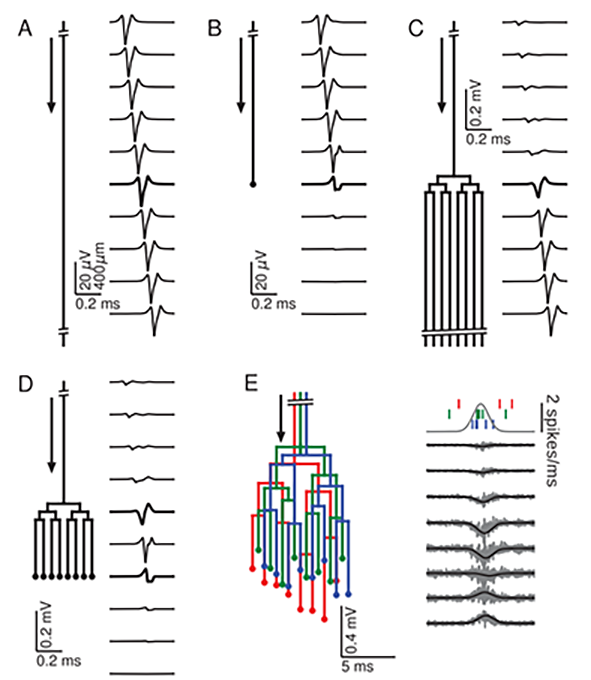
\includegraphics[width=0.7\textwidth]{Figures/Spikes/Spikes-AxonalSpikes-w100-r150}
\end{center}
\caption[]{
Text from McColgan2017: Relationship between axon morphology and extracellular potential. Multi-compartment simulations of action potentials traveling along axons with varying morphologies, as indicated by the diagram on the left-hand side of each subfigure. Action potential propagation direction indicated by arrow. Waveforms, shown on the right- hand side of each subfigure, were recorded at a horizontal distance of 150 mm from the axons. The vertical depth is indicated by the plot position, spaced by 400 mm. Horizontal plot location and distances between axons are for illustration only, all axons were simulated to lie on a straight line. (A) Action potential in a quasi-infinitely long, straight axon. (B) Terminating axon. Action potential waveform closest to the termination thickened for emphasis. (C) Branching axon. The axon branches multiple times within of 200 mm. Thicker waveform at the center of the bifurcation zone. (D) Combined bifurcations and terminations. Note the larger voltage scales in C and D, which correspond to the different number of fibers. (E) Response in a population of 100 randomized morphologies, three of which are shown schematically (colored). Activity consists of spontaneous background activity (100 spikes/s) superimposed with a brief Gaussian pulse of heightened spike rate (2000 spikes/s). Spike rate and example spike times for the three morphologies are shown at the top. Right: gray lines show activity of full population averaged over 40 trials, while the black lines show the low-pass (<1 kHz) component. Note that the time and voltage scales are different from A-D. In all graphs, spatial scales are the same, as indicated by the scale bar in A. 
\gen{Figure + caption to be updated.} Adapted from \citeasnoun**{McColgan2017}.
}
\label{fig:Spikes:AxonalSpikes}
%\figpermOurs
\end{figure}
%


\section{\blue{Effects of measurement device on spike recordings}}

In the above examples we have assumed an infinite volume conductor, that is, the extracellular conductivity
has been assumed to be the same everywhere. We have also employed
the point-electrode approximation, that is, the recording electrode has been assumed  
to record the potential at one particular position in space (\Fref{sec:VC:point-electrode}). Also it has been assumed
to faithfully record the extracellular potential without disturbing the potentials around the neuron
in any way.  As discussed in \Fref{sec:VC:electrodes}, however, real recording devices will in general affect
the measured potentials in several ways.  

\subsection{\blue{Physical sizes of contacts and shafts of recording electrode}}
\label{sec:Spikes:electrode_size}
Most electrodes presently used for extracellular recordings inside the brain consist of electrode contacts made of
highly conductive materials embedded in an electrically insulating electrode shaft. The amplitudes and shapes of 
recorded spikes are affected by the size of the electrode contacts, and as discussed in \Fref{sec:VC:disc-electrode}
this effect can be modelled by use of the disc-electrode approximation. In this approximation the spike potential is computed
by averaging results from using the point approximation across the surface of the electrode, and it is thus straightforward to implement.
 An example of its use
is provided by \Fref{fig:Spikes:electrode_size} showing spikes recorded with circular electrodes of different radii.
For one, the spike amplitude is seen to be reduced with increasing contact sizes (panel B). The spikes shape is also affected as the 
averaging of the potentials across the contact surface will reduce high-frequency components of the spike (panel C).

%%%
\begin{figure}[!ht]
\begin{center}
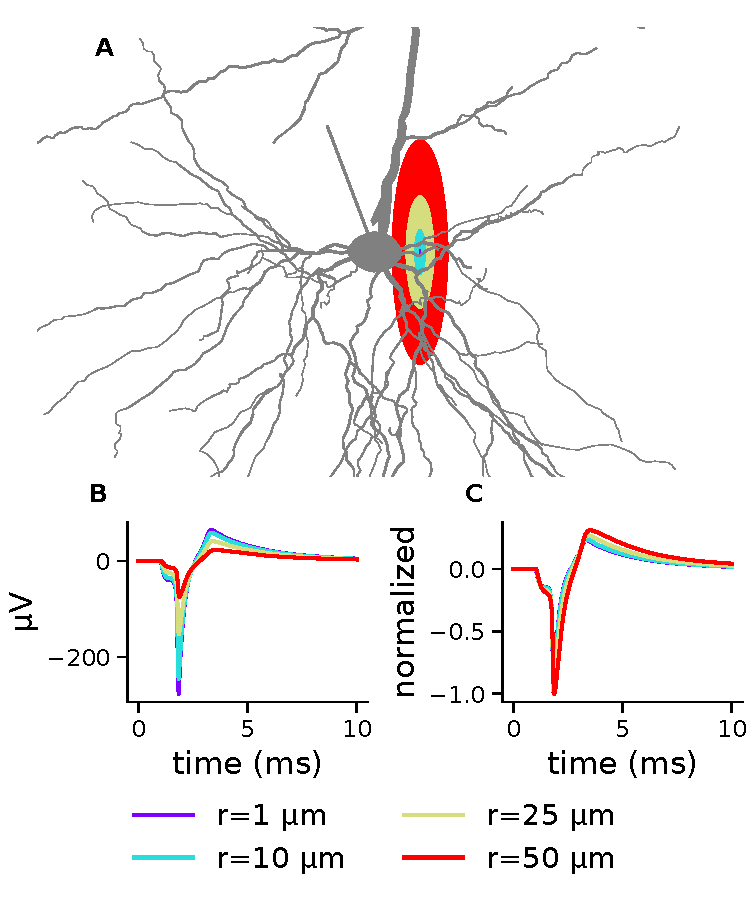
\includegraphics[width=0.6\textwidth]{Figures/Spikes/Spikes-fig_elec_size_effect.pdf}
\end{center}
\caption[]{\textbf{Effect of electrode size.}Bigger recording electrodes can cause smaller and broader EAPs.  \ghnote{Flott. Kursivere $r$? Forklare simuleringen?}
\gen{Veldig fin figur, som kanskje kan passe enda bedre here enn i VC-kapitlet "spikes" kapitlet. Hva tenker dere?}}
\label{fig:Spikes:electrode_size}
\end{figure}
%%%

The insulating electrode shaft effectively act to shadow spikes from neurons placed on the 'non-contact' side of the electrode.
Detailed studies of this requires comprehensive numerical investigations by use of FEM modeling~\cite**{Mechler2011,Mechler2012,Buccino2019}.

\subsection{\blue{Microelectrode arrays (MEAs)}}

Spikes are not only recorded in living brains. In \emph{in vitro} recordings, small slices of excised brain tissue are
placed in suitably designed dishes where physiological properties of cells and networks can be probed in detail for hours.
In so-called \emph{microelectrode arrays (MEAs)}, the bottom of the device is covered by a grid of electrode
contacts which record electrical signals generated by the neurons above. The brain slice and the MEA are both
covered with a liquid, typically saline, to protect the cells from drying out and keep them alive for the duration of the experiment, see
\Fref{fig:Spikes:MEA-setup}.

%%%
\begin{figure}[!ht]
\begin{center}
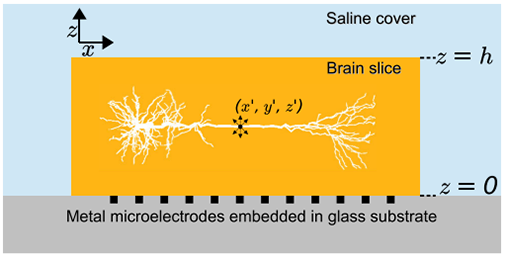
\includegraphics[width=0.7\textwidth]{Figures/Spikes/Spikes-MEA-1-w43-r300}
\end{center}
\caption[]{\textbf{MEA-setup.}
Figure is adapted from \citeasnoun**{Ness2015}.}
\label{fig:Spikes:MEA-setup}
\end{figure}
%%%

In MEAs the electrode contacts are embedded in an insulating glass plate with very 
low electrical conductivity, while the covering liquid typically has a higher electrical conductivity 
than the brain slice it covers. Thus the extracellular conductivity around the signal-generating neurons
will not be constant as assumed above, and this will affect the amplitude and shape of the recorded 
spikes. 

In general, FEM modeling will be required to solve the forward-modeling for situations such as this where
the the conductivity $\sigma$ varies with position. However, if we assume that the MEA substrate, slice and saline
all extend infinitely in the lateral directions so that $\sigma$ can be assumed to only have planar step-wise discontinuities, 
formulas analogous to \Fref{eq:XX:Vr} can be derived by use of the
\emph{method of images} from electrostatics. \gen{Referer til section i VC.}


%%%
\begin{figure}[!ht]
\begin{center}
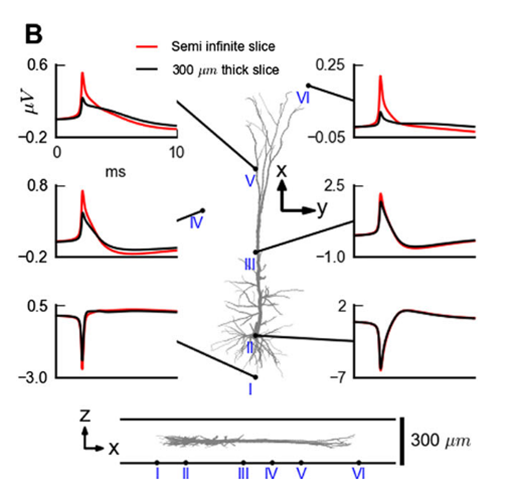
\includegraphics[width=0.8\textwidth]{Figures/Spikes/Spikes-MEA-2-w43-r300}
\end{center}
\caption[]{\textbf{MEA-spikes.}
Figure is adapted from \citeasnoun**{Ness2015}.}
\label{fig:Spikes:MEA-spikes}
\end{figure}
%%%

An example result is shown in \Fref{fig:Spikes:MEA-spikes}.
The largest effect on the spike comes from the insulating glass substrate which roughly doubles the size of the 
recorded spikes. However, also the highly-conductive 
saline cover employed in the example has an effect. More specifically, it
reduces the size of the spike compared to the hypothetical 
situation where the saline had the same value of the electrical conductivity as the brain slice.


\section{\blue{Multi-unit activity (MUA)}}

In general, a recording contact will pick up spikes from several neurons positioned in its vicinity, that is, from `multiple units'.
The term \emph{multi-unit activity (MUA)} refers to this total spiking activity seen in the high-frequency part of recorded extracellular potentials. 

%%%
\begin{figure}[!ht]
\begin{center}
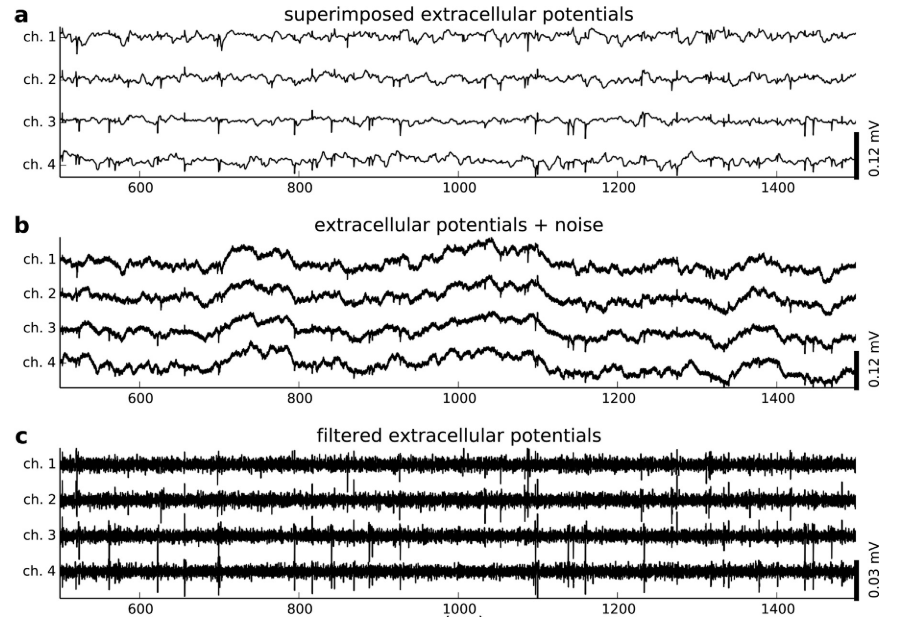
\includegraphics[width=0.8\textwidth]{Figures/Spikes/MUA-11}
\end{center}
\caption[]{\textbf{MUA tetrode}
Fra Hagen (2015):
Example benchmarking data for in vivo tetrode recordings. (a) Extracellular potential generated by population of six cortical pyramidal neurons.  
(b) Raw benchmarking data found from superposition of population potentials (from panel a) and synthesized model noise. (c) Filtered benchmarking data (corresponding to signals in (b)) showing MUA". 
Adapted from \citeasnoun**{Hagen2015}.
}
\gen{Kan vi kan legge til et panel som illustrerer en tetrode?}
\label{fig:Spikes:MUA-tetrode}
\end{figure}
%%%


\subsection{\blue{Spike extraction and sorting}}  

With only a single recording contact, the most direct way to analyse the MUA is to simply detect and count the spikes in the recorded 
signal trace. Here a suitable detection procedure must be used. This typically involves thresholding where only putative spikes larger than a 
preset threshold depending on the ambient noise level, are included. 
\gen{Kanskje vi kunne laget en enkel figur her?}

Today, spikes are typically recorded with multielectrodes, for example, 
tetrodes with four closely positioned recording contacts (\Fref{fig:Spikes:MUA-tetrode}), 
linear multielectrodes (polytrodes) with tens of contacts positioned along a straight line (\Fref{fig:Spikes:MUA-polytrode}), or 
grid-like multielectrodes with many hundred tiny contacts arranged in rectangular patterns on an electrode shaft \cite**{Jun2017}.  
On these multielectrodes, the same spike will in general show up on several contacts, and a process known as 
\emph{spike sorting}~\cite**{Quiroga2007} is required to (i) properly count spikes and (ii) to sort recorded spikes 
into contributions from individual neurons as is often the goal. 

To develop and validate methods for spike sorting, benchmarking data where the `ground truth' is known is highly desirable. Experimental benchmarking
data is hard to come by as they require simultaneous recording of intracellular action potentials and corresponding extracellular spikes.
However, model-based benchmarking data is an attractive alternative~\cite**{Einevoll2012} and the generation of such data has been pursued in several projects
\cite**{CamunasMesa2013,Hagen2015,MondragonGonzalez2017,Buccino2020}. 

An example is given in \Fref{fig:Spikes:MUA-tetrode} where virtual MUA signals
recorded by a tetrode is shown \cite**{Hagen2015}. The MUA signals have been computed by simulating six cortical neurons placed around a tetrode which are driven to spiking by a combination
of excitatory and inhibitory synaptic inputs (panel a). Further, noise with the same statistical properties as what is seen in real tetrode experiments, is added to the signal (panel b) 
prior to the high-pass filtering which results in the MUA benchmarking data (panel c). The final MUA data clearly shows how an action potential from a single neuron is seen
simultaneously as spikes on several of the tetrode contacts. 

Another example is given in \Fref{fig:Spikes:MUA-polytrode} where spikes from 16 cortical neurons are recorded by a 16-contact linear multielectode spanning the cortex. Here we observe that an action potential from a single neuron typically are observed as spikes at two to four adjacent contacts.



%%%
\begin{figure}[!ht]
\begin{center}
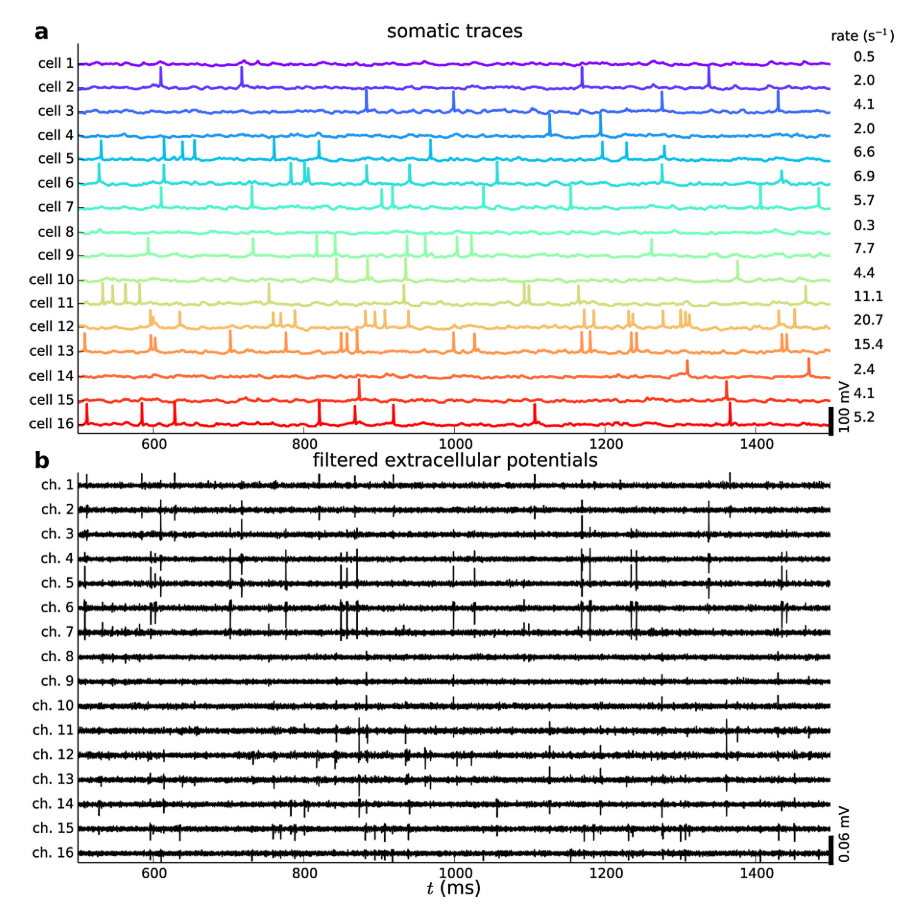
\includegraphics[width=0.8\textwidth]{Figures/Spikes/MUA-10}
\end{center}
\caption[]{\textbf{MUA linear multielectrode (polytrode)}
Fra Hagen 2015: Excerpts of intracellular and extracellular recordings for the 16 cells included in the example 16-channel polytrode benchmarking data set. 
(a) Somatic membrane potentials. Firing rates of cells 1-16 averaged over the 120 s real-time duration of the simulation are listed on the right hand side. (b) Superposition of extracellular potentials from all neurons and model noise, after band-pass filtering."
}
\gen{Kan vi kan legge til et panel som illustrerer polytroden?}
\label{fig:Spikes:MUA-polytrode}
\end{figure}
%%%

\subsection{\blue{Population firing-rate estimation from MUA}}  

The number of spikes that can be picked up above the ambient noise level by an electrode contact, depends on several factors. One is the volume density and morphological shapes of active
neurons around the contact. Another is the impedance and size of the contact itself. 
As discussed in \Fref{sec:Spikes:electrode_size} large electrode contacts will tend to reduce the spike amplitude through a spatial averaging effect, making it difficult to 
identify individual spikes from the recorded signal. If so, an estimate of the combined firing rate of the neurons surrounding the contact may be found by using the MUA signal in a different way,  that is, by rectification of the high-pass filtered extracellular potential~\cite**{Schroeder1998,Schroeder2001,Ulbert2001}. The principle behind this approach is illustrated
in \Fref{fig:Spikes:MUA-rectifify}.

%%%
\begin{figure}[!ht]
\begin{center}
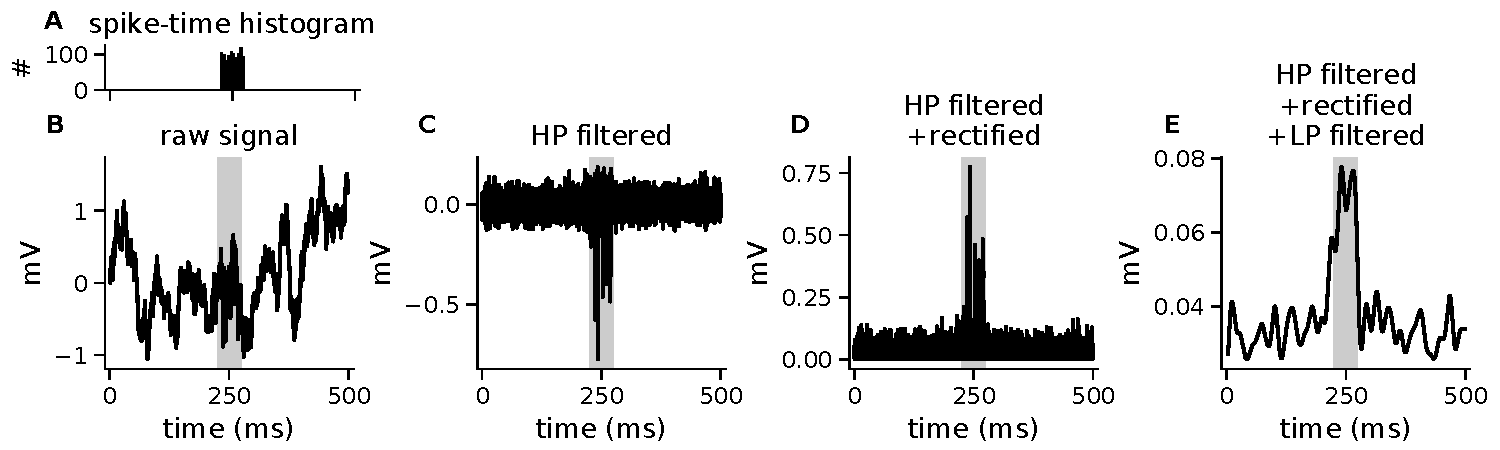
\includegraphics[width=1.\textwidth]{Figures/Spikes/fig_hay_MUA.pdf}
\end{center}
\caption[]{{\bf Illustration of MUA rectification}
{\bf A:} Spike-time histogram of the spikes to be inserted.
{\bf B:} The raw signal, containing artificially generated noise, with spikes superimposed on the signal 
according to the spike-times from {\bf A}. For each spike time the spike shape is randomly chosen from the grid in \fref{fig:Spikes:MultiCompartment}{\bf A}.
{\bf C:} High-pass filtered (>300~\si{\hertz}) version of the raw-signal in {\bf B}.
{\bf D:} Rectified version (that is, the absolute value is taken) of high-pass filtered signal in {\bf C}.
{\bf E:} Low-pass filtered (<50~\si{\hertz} version of signal in {\bf D}.
\gen{Figure illustrating principle behind MUA from rectification method}
\gen{Can you make such a figure, Torbj{\o}rn?}\tvnnote{OK?}
}
\label{fig:Spikes:MUA-rectifify}
\end{figure}
%%%

The approach was used to estimate firing rates of cortical populations of neuron in the rat barrel (somatosensory) cortex based on multielectrode laminar 
recordings~\cite**{Einevoll2007,Blomquist2009}. To test the validity of the method, a modeling study was pursued where an analogous virtual (in silico) experiment 
was performed~\cite**{Pettersen2008}. Specifically, about thousand layer-5 cortical pyramidal neurons with somas arranged in a cylindrical disc, 
mimicking a neuronal population in rat barrel cortex, was considered (\Fref{fig:Spikes:MUA-population}). The neurons received synaptic inputs simulating a volley of synaptic activation following 
sensory stimulation from flicking the appropriate whiskers. Extracellular potentials were computed for a set of contact positions along the central axis of the cylinder (\Fref{fig:Spikes:MUA-population}B).

%%%
\begin{figure}[!ht]
\begin{center}
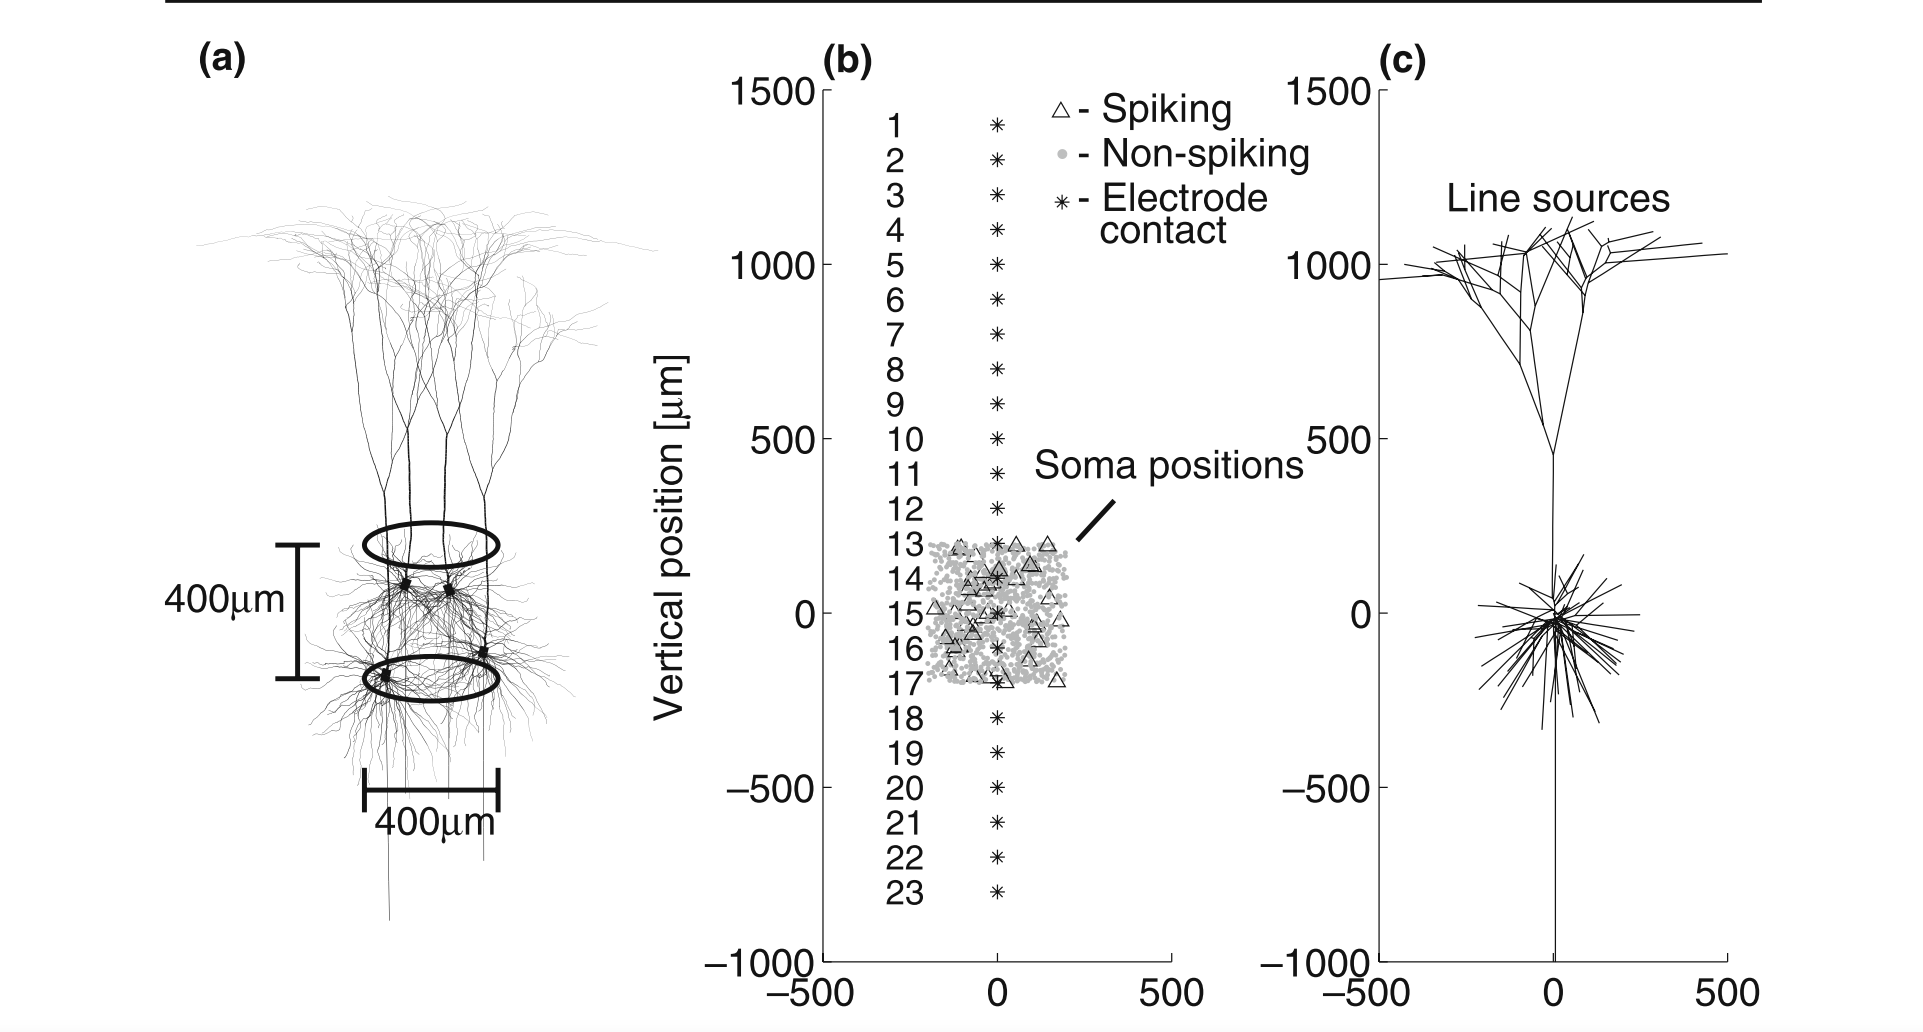
\includegraphics[width=0.8\textwidth]{Figures/Spikes/MUA-2}
\end{center}
\caption[]{
From Pettersen 2008a: \textbf{Schematic illustration of neural population created from pyramidal layer-5 neuron templates.} (b) Somas of neuronal templates are placed randomly inside a cylindrical annulus with height h=0.4 mm, outer diameter d=0.4 mm, and inner diameter 0.1 mm. One thousand cells are non-spiking (dots), while 40 cells produce a single spike following synaptic stimulation
(triangles). The electrode point contacts (stars) are aligned on the central axis of the cylindrical annulus. (c) Illustration of line-source method where the transmembrane currents passing through the 
segments of the displayed branches are modeled as line segments with uniform current density.}
\label{fig:Spikes:MUA-population}
\end{figure}
%%%

An example result is shown in \Fref{fig:Spikes:MUA-ApicalSynapses}. Here panel A shows the total extracellular potential following the synaptic activation of the population. The signal
is dominated by the low-frequency response to the synaptic input, that is, the local-field potential (LFP). The spatial pattern of the signal across recording channels reflects the
spatial distribution of synaptic inputs onto the pyramidal neurons. In this example, excitatory synapses are placed on the apical dendrites while inhibitory synapses are placed on the basal dendrites.
The dominance of low frequencies in the signal is illustrated in panel B showing the Fourier transformed signal, that is, the amplitude of each frequency component, for three of the channels.
Here it can be seen that the frequencies up to 100 Hz dominate the signal completely, that is, have the highest amplitudes (and power, corresponding to the amplitude squared). 

%%%
\begin{figure}[!ht]
\begin{center}
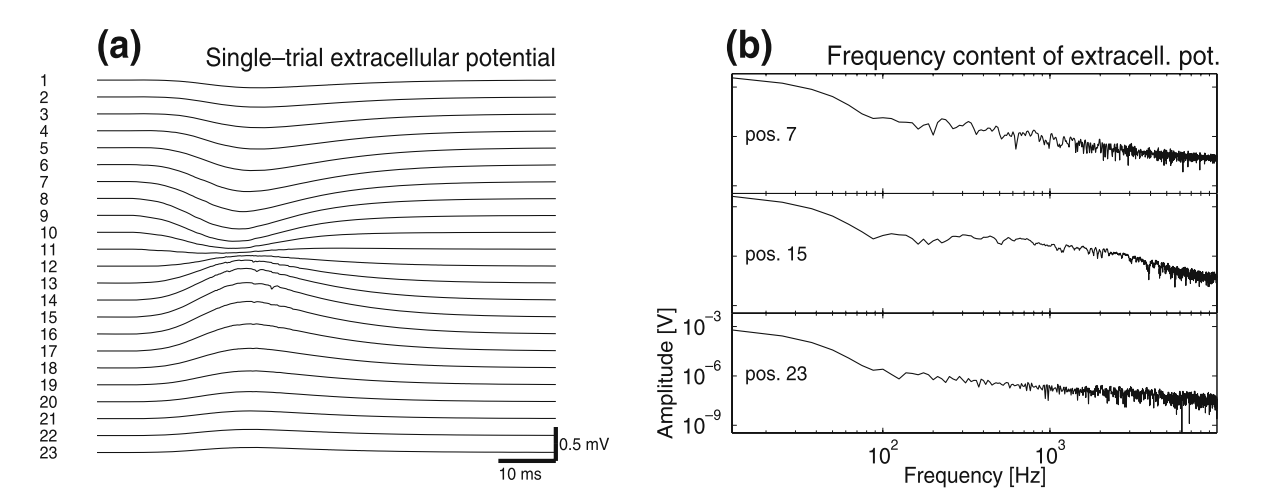
\includegraphics[width=0.8\textwidth]{Figures/Spikes/MUA-3} \\
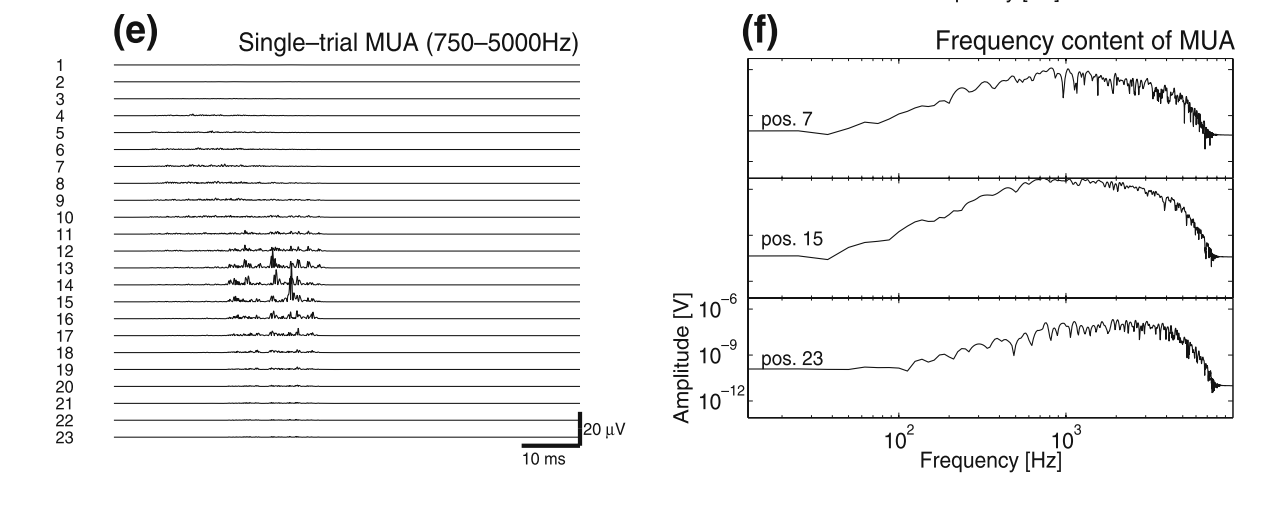
\includegraphics[width=0.8\textwidth]{Figures/Spikes/MUA-4} \\
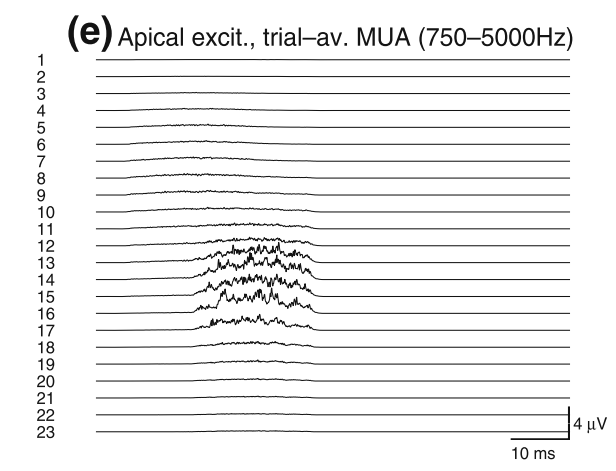
\includegraphics[width=0.4\textwidth]{Figures/Spikes/MUA-5} 
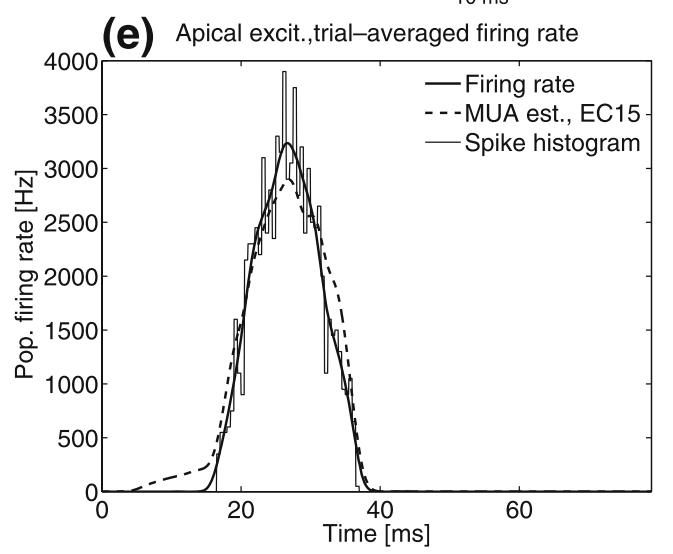
\includegraphics[width=0.4\textwidth]{Figures/Spikes/MUA-7} 
\end{center}
\caption[]{
From Pettersen 2008a: \textbf{Extracellular potentials at electrode contacts 1-- 23 for apically stimulated population.} 
(a) Single-trial raw (unfiltered) extracellular potentials. 
(b) Frequency content, i.e., Fourier amplitudes, of raw potentials in (a). 
Middle left: "(e)" MUA, i.e., high-pass filtered (750 -- 5.000 Hz) and rectified content of potentials in (a). 
Middle right "(f)" Frequency content of the MUA in (e) prior to rectification. The mean synaptic onset times are stochastically distributed around 20 ms with a standard deviation of $\sigma$=5 ms.
Lower left: "(e)": MUA, i.e., high-pass filtered (750 -- 5.000 Hz), rectified and then trial-averaged signals for apically excited population. 
Lower right: "(e)": Spike histogram (bin width 0.5 ms), `true' population firing rate, and estimated firing rate from the MUA of electrode contact 15. The amplitude of the estimated firing rate
has been fitted to minimize the relative mean square deviation er  between the estimated and `true' population firing rates. 
\gen{Refer to Pettersen2008 for detailed explanation.}
}
\label{fig:Spikes:MUA-ApicalSynapses}
\end{figure}
%%%

While the spikes are buried by the low-frequency components in the raw signal, they can be extracted by high-pass filtering 
and subsequent rectification. Results are shown in \Fref{fig:Spikes:MUA-ApicalSynapses}, as a function of time in panel C
and in frequency space in panel D. \gen{Panel labeling is wrong in present figures}
A first observation in panel C is
that the remaining signal is confined to channels deep in the cortex, that is, close to the somas of the neurons in the populations.
This reflects that extracellular signatures of action potentials are typically confined to within 100~$\mu$m from the soma, cf. \Fref{fig:Spikes:DifferentNeuronModels}. A second observation in panel C is that the MUA signals 
only last for about 20~ms, which turns out to be the time period in which the neurons in the model fire action potentials~\cite**{Pettersen2008}.
A third observation is that the MUA signal is not smooth, but `noisy' in the sense that it
consists of a collections of sharp peaks of different heights. This `noisiness' stems from the inherent randomness both in the times of spiking 
and the positions of the somas of the low number (40) of spiking neurons in the population. 

In sensory systems it has been common to measure 
trial-averaged responses, that is, the response averaged over many repetitions of the same stimulus. The rationale is that this procedure highlights the contributions from sensory input in that the effects of other synaptic inputs and noise in sensory neurons are reduced. The trial-averaged MUA found from averaging MUA results from forty model trials, is shown in 
panel E of \Fref{fig:Spikes:MUA-population}, revealing a much less `noisy' signal. 

The obvious next question is to what extent the resulting MUA signal gives a good measure of the population firing rate. Unlike in experiments, the true underlying firing rate is known in the model, allowing for a quantitative comparison. The question was studied in detail for the model in question in \citeasnoun**{Pettersen2008}. The noisyness of MUA signals from individual trials (\Fref{fig:Spikes:MUA-population}C) did not allow for accurate estimation of firing rates in individual trials. However, accurate estimates for trial-averaged firing rates (commonly referred to as Post Stimulus Time Historgrams (PSTHs)) could be obtained from trial-averaged MUA signals. 
An example is given in \Fref{fig:Spikes:MUA-ApicalSynapses}F. Here a firing-rate estimate based on the MUA signal from one of the recording channels positioned at a depth in the midst of somas of the population is compared with the true, temporally smoothed firing rate.  
The overall agreement is observed to be quite good.

 One deviation is that the MUA signal predicts a non-zero firing rate prior to the onset of true firing, the reason being that the synaptic input current itself gives a contribution to the MUA signal. Another deviation is that the MUA-based firing rate predicts a too low maximum firing rate, due to cancellations of signal contributions from temporally overlapping spikes from different neurons. This latter effect increases with increasing firing rates and can be remedied by assuming a supralinear relationship between the MUA signal and firing rate \cite**{Pettersen2008}.  The accuracy of the population firing rate can also be improved by using MUA signals from several adjacent recording channels in the estimation \cite**{Pettersen2008}.  
 
The accuracy of this MUA-based estimation of population firing rates will depend on the specific situation considered. In \citeasnoun**{Pettersen2008}, it was, for example, found
that the prediction was slightly more accurate when the population in \Fref{fig:Spikes:MUA-population} is driven by excitatory inputs onto the basal dendrites rather than onto the
apical dendrites as in \Fref{fig:Spikes:MUA-ApicalSynapses}.
 
%
%%%%
%\begin{figure}[!ht]
%\begin{center}
%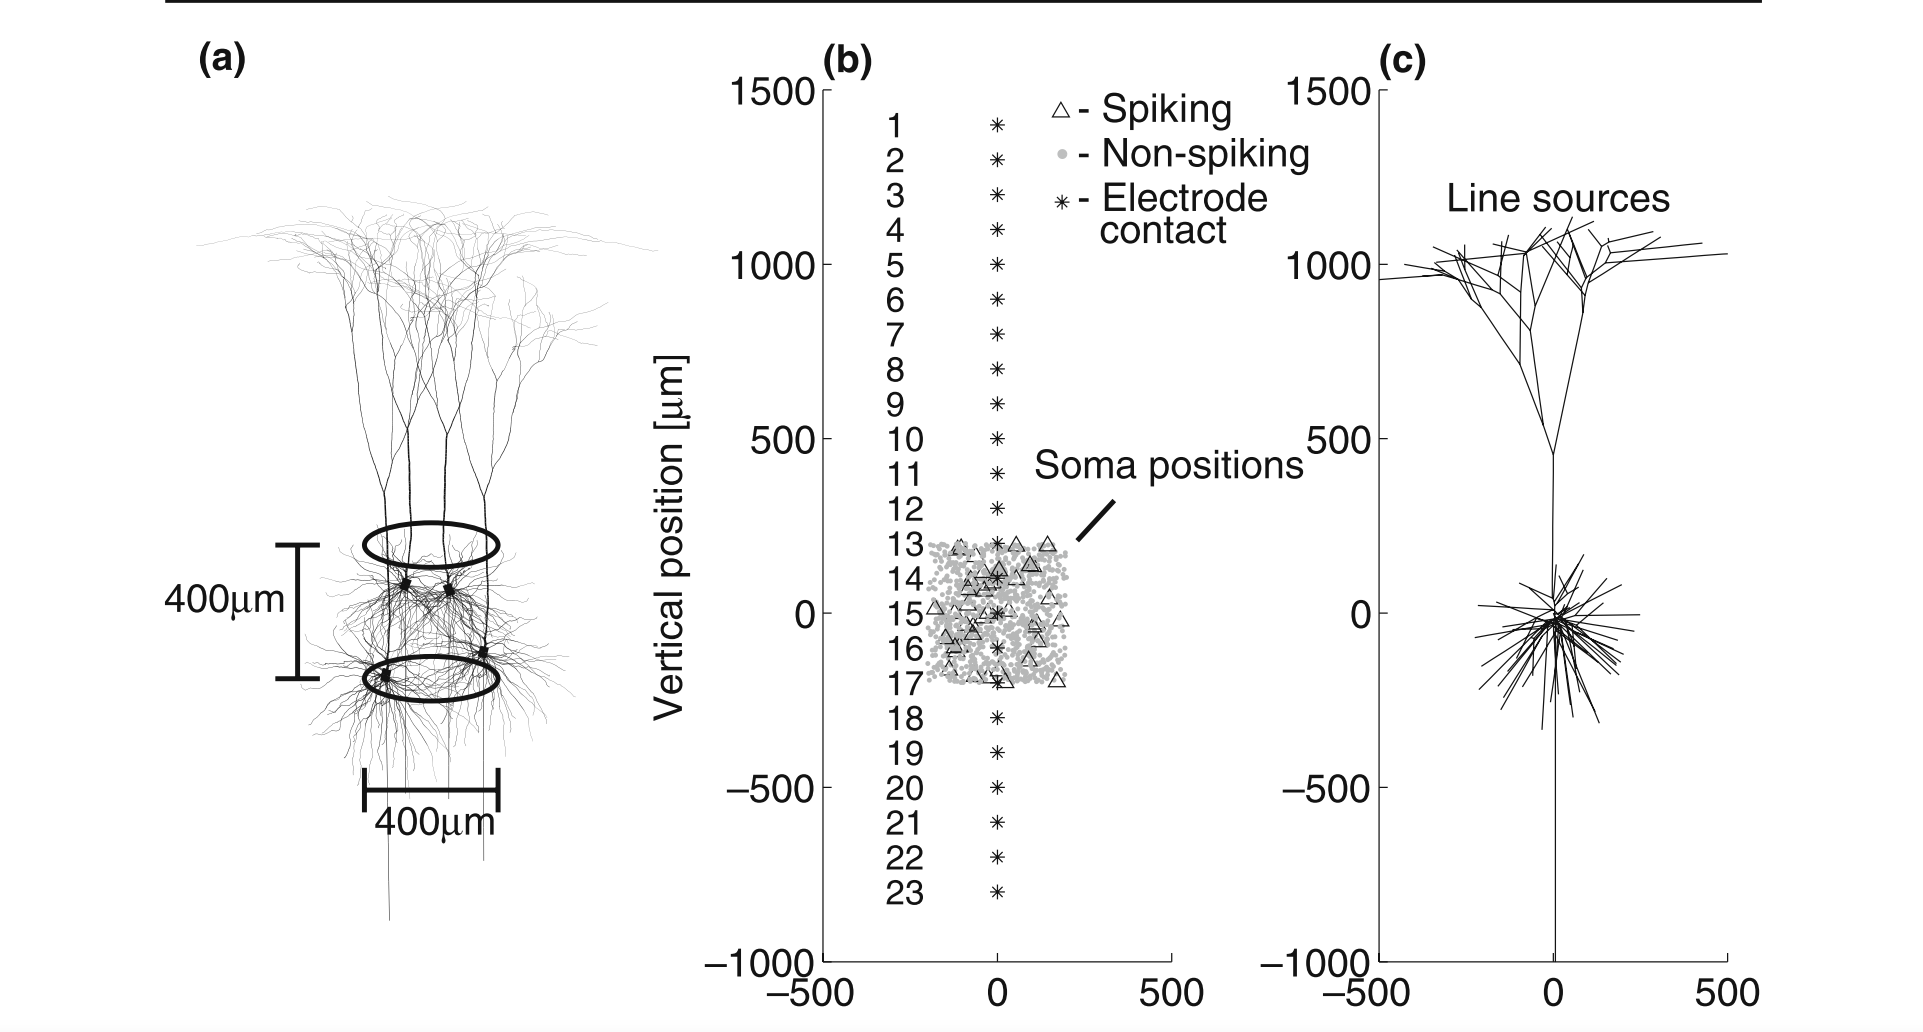
\includegraphics[width=0.8\textwidth]{Figures/Spikes/MUA-2}
%\end{center}
%\caption[]{\textbf{MUA}}
%\label{fig:Spikes:MUA-A}
%\end{figure}
%%%%
%

%
%%%%
%\begin{figure}[!ht]
%\begin{center}
%\includegraphics[width=0.4\textwidth]{Figures/Spikes/MUA-6}\\
%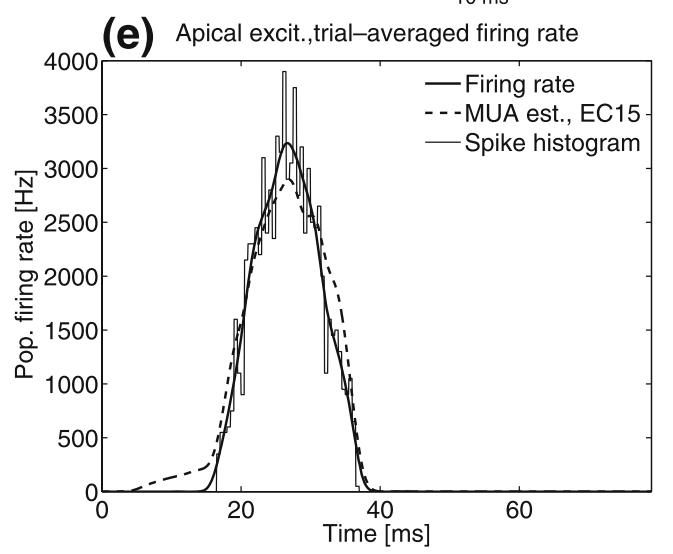
\includegraphics[width=0.4\textwidth]{Figures/Spikes/MUA-7}
%\end{center}
%\caption[]{\textbf{MUA}}
%\label{fig:Spikes:MUA-C}
%\end{figure}
%%%%
%
%%%%
%\begin{figure}[!ht]
%\begin{center}
%\includegraphics[width=0.8\textwidth]{Figures/Spikes/MUA-8}
%\end{center}
%\caption[]{\textbf{MUA}}
%\label{fig:Spikes:MUA-D}
%\end{figure}
%%%%
%

%\section{\red{Insights from MUA studies}} 
%\ghnote{I added this kind of subsection to most of the Part 2 - sections. I thought it might be an idea to finish the MUA, LFP, ECoG and EEG sections with summaries of what these modalities typically tell us, i.e. in terms of (i) what aspects of neural activity they reflect (spikes, synaptic inputs, dendritic ion channels, which ion channels, which kind of neurons, something on network structure, cell orientation, cortical folding etc.), and what what they can tell us about cognitive states (attentive, drowsy etc.). I am not sure about this idea, though. Maybe it will be too challenging to get an overview over the literature - we dont want to put the entire Nunez-book into the EEG-chapter.}

%%%%%%%%%%%
%% Box: Spike sorting
%%%%%%%%%%%
%%\begin{boxfloat}{Spike sorting}
%%  \label{mm:box:spike-sorting}
%\subsection{\red{Box: Spike-sorting}}
%\gen{This was a Box in the Sterratt chapter}
%%
%\centerline{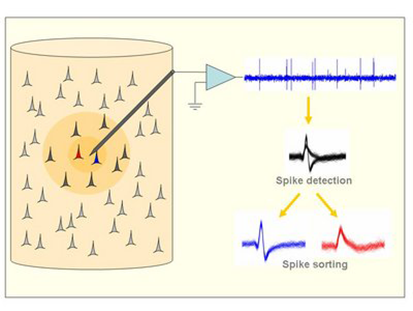
\includegraphics{Figures/Spikes/Spikes-sorting-w35-r300}}\vspace*{6pt}
%%
%A sharp electrode placed in brain tissue will pick up spiking signals from several neurons. 
%However, the shapes of the spikes will be different for the different neurons, and this can be used to sort the spikes according to their neurons of origin. This is referred to as \index{spike sorting}, 
%and is a problem of great practical importance both for neuroscience research and development of neuroprosthetic devices. 
%
%In the present day with electrodes with hundreds or thousands of electrode recording contacts, fast and accurate automatic spike-sporting methods are needed to replace time-consuming manual spike-sorting methods~\cite**{Quiroga2007}. To develop and test such automatic methods, one needs
%benchmarking spiking data where the `ground truth', that is, the actual spiking times for the contributing neurons, is known~\cite**{Einevoll2012}.
%One use of the EP modelling scheme for spikes has been to generate such benchmarking data~\cite**{CamunasMesa2013,Hagen2015,MondragonGonzalez2017}. 
%
%Modern electrodes have numerous recording contacts, often placed only some micrometers apart. Thus a spike can be measured at several contacts
%simultaneously, each contact recording a slightly different shape reflecting the different positions of the contacts relative to the spiking neuron. 
%This not only allows for accurate spike sorting, but also for estimation of the spatial position of the neuron. Likewise, the spatial variation of the 
%spike shape around the neuronal soma (see Figure~\Fref{fig:Spikes:MultiCompartment}) 
%depends on the details of the intracellular action potential and dendritic morphology thus also allowing for the 
%identification of neuron type~\cite**{Buccino2018}.    
%\gen{Figure to be adapted from Quiroga (2007).}
%%\end{boxfloat}
%%%%



%While the formulae above were derived for a neuron model with a single passive dendritic stick, similar expressions can be derived for 
%more complicated neuron models where several passive sticks protrude from the soma, see \citeasnoun**{Pettersen2008}.
%The main conclusions above hold also for these neuron models, in particular that spike widths always increase with distance and that
%the amplitude of a spike is proportional to $d^{k}$ where $k\sim1.5-2$. For neurons with many dendrites attached to the 
%soma, the contributions to the spike amplitude roughly adds up. A simple rule of thumb is that a neuron's spike amplitude is 
%roughly proportional to the sum of the cross-sectional areas for all dendrite branches attached directly onto to the soma. Neurons with many thick
%dendritic branches attached to the soma will thus generate the largest spikes. See~\citeasnoun**{Pettersen2008} for further discussion.
%
%
%{\bf TEXT COPIED FROM STERRATT CHAPTER ON 2020-10-13}
%
%\section{Dependence of spike size and shape on neuronal properties}
%
%Extracellular measurement of spikes from a neuron in living brains is blind in the sense that it is
%not known what type of neuron is recorded from when an electrode is lowered into the brain.
%Some neuron types produce spikes with larger amplitudes and/or broader shapes than
%others,
%%
%%\todo{TVN: Nevne at det ofte sorteres i "putative excitatory" og "putative inhibitory"?}
%%
%and as seen in Figure~\Fref{mm:fig:EP-spike-MultiCompartment} both the shape and amplitude 
%depend critically on recording positions. Large spike amplitudes imply that they will be more dominant in electrical recordings,
%and ideally this bias should  be considered in the analysis of joint recordings 
%of spikes from many neurons. 
%
%To understand the link between the morphology of neurons and their spike amplitudes and shapes
%it is convenient to consider ball-and-stick neurons where a passive dendrite cable `stick' is connected to a point-like soma.
%Despite its simplicity, the ball-and-stick neuron model exhibits the key qualitative features observed in
%Figure~\Fref{mm:fig:EP-spike-MultiCompartment} when the multi-compartmental EP formula in 
%\Fref{mm:equation:Ve-multi-compartment}
%is used; that is, rapid attenuation of spike amplitude and increased spike width as the distance from the soma 
%increases \cite**{Pettersen2008,Pettersen2012}. 
%
%\citeasnoun**{Pettersen2008} took advantage of the mathematical tractability of the ball-and-stick model to
%derive analytical expressions for how the amplitude of the recorded spike depends on distance from the neuron as well
%as the electric properties of the neuron. The action potentials were decomposed into contributions from
%many frequency components and each frequency component was considered individually.
%This is illustrated in Figure~\Fref{mm:fig:EP-spike-ball-and-stick-frequency} where the amplitudes of the different frequency components needed to
%represent the intracellular action potential (membrane potential) and extracellular spike respectively are shown.
%A key observation here is that for the extracellular spike, the largest contributions comes from frequencies larger than 100~hertz.
%%%%%%%%%%%
%% Figure: Action potential and its frequency content
%%%%%%%%%%%
%%\begin{cnfigure}{Figures/fig-not-pushed-to-github}
%%\begin{cnfigure}{Figures/mm/EP-spike-ball-and-stick-frequency-w90-r150}
%%\caption[]{
%%Frequency content of example intracellular (a) and extracellular spike (b).
%%%
%%%(a) Action potential used in simulations in Figure~\Fref{mm:fig:EP-spike-ball-and-stick-results}(inset) 
%%%\todo{Comment from DCS not understood.}
%%%and its frequency content. 
%%%%The intracellular spike width is defined as the
%%%%width of the AP at half amplitude and is 0.55~ms for the standard
%%%%AP, and half the value for the narrow AP. 
%%%(b) Frequency content of example extracellular spike.
%%%Inset: Typical spike shape computed a distance $r=10~\mu$m
%%%perpendicular to the dendrite at the level of soma for a ball-and-stick 
%%%neuron with diameter $d=2~\mu$m and infinite dendrite length.
%%%Here the intracellular action potential in left panel was imposed as a voltage-clamp in the soma.
%%%The extracellular spike width is defined as the width of the negative phase at 25\% of its maximum
%%%amplitude and is 0.44~ms for the example spike.
%%%The amplitude (peak-to-peak value) of the spike is $56~\mu$V  
%%\todo{Figure + caption to be updated. Will only include standard AP in final figure.} 
%%Adapted from \citeasnoun**{Pettersen2008}.
%%}
%%\label{mm:fig:EP-spike-ball-and-stick-frequency}
%%\figpermOurs
%%\end{cnfigure}
%
%
%%\todo{Explain the idea that the question is about how currents entering the soma during the AP returns through the dendrite}
%
%\citeasnoun**{Pettersen2008} derived simple formulae relating the intracellular action potential to the extracellular spike for two limiting cases:
%when the recording is done near to the soma or far away from the soma. For recordings near the soma the 
%amplitude $|\hat{V}_\mathrm{e,near}(f,\vec{r})|$ of the spike signal for each frequency component with frequency $f$ was found to be approximated
%by
%%
%\begin{equation}
%  |\hat{V}_\mathrm{e,near}(f,\vec{r})| 
%  \propto \frac{d^{3/2}}{r} \sqrt{ \frac{f C_\mathrm{m}}{R_\mathrm{a}} }  |\hat{V}_\mathrm{s}(f)| 
%  \label{mm:equation:Ve_near}
%\end{equation}
%%
%Here $|\hat{V}_\mathrm{s}(f)|$ is the amplitude of frequency component of the soma membrane potential at the same
%frequency (see Figure~\Fref{mm:fig:EP-spike-ball-and-stick-frequency}).
%For recording positions far away from the soma, the following expression was instead found:
%%%%
%\begin{equation}
%  |\hat{V}_\mathrm{e,far}(f,\vec{r})|  \propto d^{2} \frac{|\cos \theta| }{r^2  R_\mathrm{a}}  |\hat{V}_\mathrm{s}(f)| 
%  \label{mm:equation:Ve_far}
%\end{equation}
%%%%
%In these formulas, $d$ is the diameter of the dendritic
%stick, $C_\mathrm{m}$ the specific membrane capacitance, and $R_\mathrm{a}$ the specific axial resistance.  
%

%%%%%%%%%%%
%% Figure: Spike widths and amplitudes
%%%%%%%%%%%
%\begin{cnfigure}{Figures/mm/EP-spike-ball-and-stick-results-w100-r150}
%\caption[]{
%Spike widths (left) and (peak-to-peak) spike amplitudes (right) as a function of
%distance from soma for a detailed pyramidal cell model (pyramidal) and two
%types of ball-and-stick models: long, finite ball-and-stick
%model (fin.~stick, long) with diameter $d=2~\mu$m and length
%$l=1$~mm and a short, finite ball-and-stick model (fin.~stick, short) with diameter $d=1~\mu$m and length $l=0.2$~mm,
%see Figure~\Fref{mm:fig:EP-spike-ball-and-stick-neuron-models}.
%The intracellular action potential shown in the inset in the left panel of 
%Figure~\Fref{mm:fig:EP-spike-ball-and-stick-frequency} was imposed as a voltage-clamp in the soma.
%The EP was recorded in the
%somatic plane normal to the stick/primary apical dendrite. 
%In right panels guidelines illustrating the power-law decays $1/r$ and
%$1/r^{2}$ have been added. 
%For further details see \citeasnoun[Figure 6]{Pettersen2008}.
%\todo{Figure + caption to be updated. Adapted from \citeasnoun**{Pettersen2008}.}
%}
%\label{mm:fig:EP-spike-ball-and-stick-results}
%\figpermOurs
%\end{cnfigure}


%\paragraph{Spike amplitude dependence on distance}

%%%%%%%%%%%%%%%%%%%%%%%%%%%
%% Box: Spike sharpness
%%%%%%%%%%%    
%\begin{boxfloat}{Spike sharpness}
%  \label{mm:box:spike-sharpness}
%There are several qualitative insights regarding the sizes and widths of spikes that can 
%be found from the near-field and far-field formulae in Equations~\Fref{mm:equation:Ve_near} and 
%\Fref{mm:equation:Ve_far}, respectively. One relates directly to the shape of the spike:
%in the near-field expression, the high-frequency components of the spike is amplified 
%compared to the low-frequency components, that is, $\hat{V}_\mathrm{e,near}(f,r) \propto \sqrt{f}$.
%Thus close to the soma the spike is observed to be sharper than the intracellular action potential
%as observed in the insets in Figure~\Fref{mm:fig:EP-spike-ball-and-stick-frequency}. 
%In the far-field regime there is no such high-frequency amplification ($\hat{V}_\mathrm{e,near}(f,r) \propto f^0 \sim 1$).
%As a consequence, spikes measured far away from the soma will have less high-frequency content than those measured close to soma.
%Thus the far-away spikes will be blunter and have larger spike widths as seen in the spike-width panel of 
%Figure~\Fref{mm:fig:EP-spike-ball-and-stick-results}.
%%
%%\centerline{\includegraphics{Figures/mm/MEA-1-w43-r300}}\vspace*{6pt}
%%
%\end{boxfloat}
%%%%%%%%%%%%%%%%%%%%%%%%%%%%%%%%





%
%%%%%%%%%%%
%% Sidebox: Fourier sum
%%%%%%%%%%%
%\begin{sidebox}
%Time signals, such as the time course of a spike $V_\mathrm{e}(t)$,  can conveniently 
%be represented as a sum of \firstterm{Fourier components} with different frequencies $f$. 
%Such a Fourier sum can be constructed in
%various ways. The derivations in 
%Section~\Fref{mm:sec:spike-widths-amplitudes}, building on \citeasnoun**{Pettersen2008}, use the  
%convention that a time signal $S(t)$ is the real part of the complex sum $\sum_{f}  \hat{S}(f) \exp (j 2 \pi f t)$. 
%Here $j$ is the unit of imaginary numbers, and  $\hat{S}(f)$ is in general a complex number. 
%\end{sidebox}
%%
%
%%%%%%%%%%%
%% Figure: Spike widths and amplitudes
%%%%%%%%%%%
%\begin{cnfigure}{Figures/mm/EP-spike-ball-and-stick-results-w100-r150}
%\caption[]{
%Spike widths (left) and (peak-to-peak) spike amplitudes (right) as a function of
%distance from soma for a detailed pyramidal cell model (pyramidal) and two
%types of ball-and-stick models: long, finite ball-and-stick
%model (fin.~stick, long) with diameter $d=2~\mu$m and length
%$l=1$~mm and a short, finite ball-and-stick model (fin.~stick, short) with diameter $d=1~\mu$m and length $l=0.2$~mm,
%see Figure~\Fref{mm:fig:EP-spike-ball-and-stick-neuron-models}.
%The intracellular action potential shown in the inset in the left panel of 
%Figure~\Fref{mm:fig:EP-spike-ball-and-stick-frequency} was imposed as a voltage-clamp in the soma.
%The EP was recorded in the
%somatic plane normal to the stick/primary apical dendrite. 
%In right panels guidelines illustrating the power-law decays $1/r$ and
%$1/r^{2}$ have been added. 
%For further details see \citeasnoun[Figure 6]{Pettersen2008}.
%\todo{Figure + caption to be updated. Adapted from \citeasnoun**{Pettersen2008}.}
%}
%\label{mm:fig:EP-spike-ball-and-stick-results}
%\figpermOurs
%\end{cnfigure}
%
%%%%%%%%%%%
%% Figure: Frequency-dependent distribution of return currents
%%%%%%%%%%%
%\begin{cnfigure}{Figures/mm/EP-spike-ball-and-stick-sketch-w70-r300}
%%\begin{cnfigure}{Figures/fig-not-pushed-to-github}
%\caption[]{Illustration of ball-and-stick neuron and its frequency-dependent 
%distribution of dendritic return currents following injection of a sinusoidal current into the soma.
%The net current entering the soma will enter the dendrite as an axial current, and return to the 
%ECS via the dendrite membrane. The inset shows the spatial distribution of this return current
%for different frequencies. The higher the frequency, the closer the return currents will be and
%the smaller the frequency-dependent length constant $\hat{\lambda}(f)$, reflecting the weighted mean 
%of the return-current positions (see sidebox), will be. 
%\todo{Figure + caption to be updated. Adapted from \citeasnoun**{Pettersen2012}.}
%\todo{June 2019: Move inbset to Ch. 5?}
%}
%\label{mm:fig:EP-spike-ball-and-stick-sketch}
%\figpermOurs
%\end{cnfigure}
%%
%
%
%
%%%%%%%%%%%
%% Box: Ball-and-stick model for spikes
%%%%%%%%%%%
%\begin{boxfloat}{Ball-and-stick model for spikes}
%  \label{mm:box:ball-and-stick-spikes}  
%To understand the dependence of spike shapes and amplitudes on model parameters for the ball-and-stick neuron, it is useful
%to consider the EP set up by each of the frequency (Fourier) components of the action potentials separately. 
%For recording positions $\vec{r}$ very close to the soma, the contribution from the soma current will dominate over the contributions from the dendrite 
%in the sum giving the EP in \Fref{mm:equation:Ve-multi-compartment}. Then the amplitude of the
%predicted oscillating EP $|\hat{V}_\mathrm{e,near}(f,\vec{r})|$ is approximately given by 
%%
%\begin{equation}
%  |\hat{V}_\mathrm{e,near}(f,\vec{r})| = \frac{|\hat{I}_\mathrm{s}(f)|}{4 \pi \sigma r} 
%  \label{mm:box:equation:Ve_near_1}
%\end{equation}
%%
%where $|\hat{I}_\mathrm{s}(f)|$ is the amplitude of the oscillating current through the soma membrane.
%%and also the axial current entering the dendrite from the soma compartment. 
%For the relatively high frequencies of most relevance for the spike, this soma current is related to the soma membrane potential 
%$\hat{V}_\mathrm{s}(f)$ through~\cite**{Pettersen2008}
%%
%\begin{equation}
%  |\hat{I}_\mathrm{s}(f)| =  \frac{\pi^{3/2} d^{3/2}}{\sqrt{2}} \sqrt{ \frac{f C_\mathrm{m}}{R_\mathrm{a}} }  |\hat{V}_\mathrm{s}(f)|
%  \label{mm:box:equation:Isoma}
%\end{equation}
%%
%and the spike EP is thus found to be
%%
%\begin{equation}
%  |\hat{V}_\mathrm{e,near}(f,\vec{r})| 
%  = \frac{\sqrt{\pi}}{4 \sqrt{2} \sigma}
%     \frac{d^{3/2}}{r} 
%     \sqrt{ \frac{f C_\mathrm{m}}{R_\mathrm{a}} }  |\hat{V}_\mathrm{s}(f)| 
%  \propto \frac{d^{3/2}}{r} \sqrt{ \frac{f C_\mathrm{m}}{R_\mathrm{a}} }  |\hat{V}_\mathrm{s}(f)| 
%  \label{mm:box:equation:Ve_near_2}
%\end{equation}
%%
%\todo{June 2019: Coordinated with or moved to Ch. 5.}
%%
%For recording positions further away from the soma, the contribution from return membrane currents must be taken into
%account in the sum in \Fref{mm:equation:Ve-multi-compartment}. An approximate way of doing this is to
%assume all return currents to leave the dendrite at a single height $\lambda_\mathrm{AC}(f)$ above the soma, where 
%this frequency-dependent length constant corresponds to the weighted mean of the positions of the return currents along
%the dendrite stick. (The subscript `AC' denotes `alternating current'.)
%Then the EP can be approximated by using the 
%dipolar expression in \Fref{mm:equation:Ve-dipole-p}, that is,
%%%%
%\begin{equation}
%  |\hat{V}_\mathrm{e,far}(f,\vec{r})| =  \frac{|p(f) \cos \theta|}{4 \pi \sigma r^2} 
%                                            = \frac{| \hat{I}_{s}(f) \lambda_\mathrm{AC}(f) \cos \theta|}{4 \pi \sigma r^2}   
%                                                                                        \label{mm:box:equation:Ve_far_1}
%\end{equation}
%%%%
%One way to define an AC length constant is as the mean value of the 
%envelope of the sinusoidally varying (normalized) membrane current
%$\hat{i}_\mathrm{m}$ weighted with distance $z$ from soma, 
%see Figure~\Fref{mm:fig:EP-spike-ball-and-stick-sketch}. 
%For an infinite dendrite stick this corresponds to
%%
%\begin{equation}
%  \lambda_\mathrm{AC}^\infty(f) = \frac{\int_0^\infty z |\hat{i}_\mathrm{m}| dz}{\int_0^\infty |\hat{i}_\mathrm{m}| dz} 
%\nonumber
%%=  \frac{\sqrt{2}\lambda}{\sqrt{\sqrt{W^2+1}+1}}.
%\end{equation}
%%
%
%For high frequencies ($f \gg 1/2 \pi R_\mathrm{m} C_\mathrm{m}$) this is after some algebra 
%found to give (see \citeasnoun[Appendix C]{Pettersen2008} for details)
%%
%\begin{equation}
% \lambda_\mathrm{AC}^\infty(f) =  \frac{\lambda}{\sqrt{\pi f \tau}} = 
%  \frac{1}{2\sqrt{\pi}} \sqrt{\frac{d}{f R_\mathrm{m} C_\mathrm{m}}}
%\label{mm:box:equation:approx_lambda_ac}
%\end{equation}
%%
%where $\lambda$ is the cable length constant from 
%%Chapter~\Fref{XX:chap:XX}
%Chapter~5. f{REF} 
%
%%










